\documentclass[12pt, a4paper, twoside]{book}

\usepackage[sorting=none,citestyle=ieee,backend=biber]{biblatex}
\bibliography{bibliography}

\usepackage[usenames,dvipsnames,table]{xcolor}
\usepackage[bitstream-charter]{mathdesign}
\usepackage{fancyhdr}
\usepackage[colorlinks]{hyperref}
\hypersetup{
     colorlinks   = true,
     allcolors    = blue
}

\usepackage[nogroupskip,nonumberlist,toc]{glossaries}
\makeglossaries

\usepackage{amsmath}
\usepackage{minted}
\usemintedstyle{pastie}

\usepackage{fancyhdr}
\usepackage{tikz}
\usetikzlibrary{trees}
\usepackage{pgfgantt}
\usepackage{graphicx}
\usepackage{tabularx}
\graphicspath{{Graphics/}}
\usepackage[]{algorithm2e}

\usepackage{enumitem}
\usepackage{parskip}
\usepackage{pdfpages}
\usepackage{rotating}
\usepackage{setspace}
\usepackage{pgfplots}
\usepackage{pgfplotstable}
\usepackage{longtable}
\usepackage{tabu}
\usepackage{booktabs}
\usepackage{caption}
\usepackage{threeparttable}
\usepackage{filecontents}
\usepackage[hmarginratio=3:2]{geometry}
\usepackage{tocloft}
\usepackage[toc,page]{appendix}
\renewcommand{\cftpartleader}{\cftdotfill{\cftdotsep}}
\renewcommand{\cftchapleader}{\cftdotfill{\cftdotsep}}

\renewcommand{\baselinestretch}{1.5} % 1.5 line spacing

% Define acronyms
% Example definition:
% \newacronym{fpga}{FPGA}{Field-programmable Gate Array}
\newacronym{vr}{VR}{Virtual Reality}
\newacronym{hmd}{HMD}{Head-mounted Display}
\newacronym{hci}{HCI}{Human-computer Interaction}
\newacronym{sdk}{SDK}{Software Development Kit}
\newacronym{vrida}{VRIDA}{Virtual Reality Interior Design Applications}
% End acronyms

\pgfplotsset{compat=1.13}
\raggedbottom

\begin{document}

\frontmatter

% Title page horizontal line
\newcommand{\HRule}{\rule{\linewidth}{0.5mm}}

% Title of report
\newcommand{\ttitle}{Architectural Design and Visualisation in Virtual Reality}

\begin{titlepage}
    \begin{center}
        \begin{figure}[ht]
            \centering
            
\includegraphics[width=4cm]{crest.jpg}
        \end{figure}
        
        \textsc{\LARGE University of Warwick}\\[0.25cm]
        {\Large{Department of Computer Science}}\\[1.5cm]
        \HRule \\[0.4cm]
        {\huge \bfseries \ttitle}\\
        \HRule \\[1.5cm]
        
        \begin{minipage}{0.4\textwidth}
            \begin{flushleft}
                \large \emph{Authors:}\\Alex Dixon,\\David Richardson,\\Jakub Zawadzki
            \end{flushleft}
        \end{minipage}
        \begin{minipage}{0.4\textwidth}
            \begin{flushright}
                \large \emph{Supervisors:}\\Dr. Arshad Jhumka,\\Dr. Hongkai Wen\\
                \large \emph{Secondary Marker:}\\Dr. Ligang He
            \end{flushright}
        \end{minipage}\\[1cm]
        
        \textit{\large CS407 Group Project Report}\\
        {\large Summer 2017}\\
        
        \vfill
    \end{center}
\end{titlepage}

% Blank pages for 
\pagestyle{empty}

\newgeometry{hmarginratio=2:3}

% Clear page headers
\fancyhead{}
\fancyhead[LO]{\leftmark}
\fancyhead[RE]{\leftmark}
\setlength{\headheight}{15pt}
\renewcommand{\headrulewidth}{0.4pt}
\renewcommand{\footrulewidth}{0.4pt}
\renewcommand{\chaptermark}[1]{%
\markboth{#1}{}}
% End clear page headers

\chapter{Abstract}

% High quality virtual reality systems have recently exploded onto the mainstream market for consumers, opening up new means for human-computer interaction. Research into the use of these new devices in commercial and industrial applications has also begun to take up traction. This project aimed to create a virtual reality-based tool for the creation of 3D spaces

TODO

\clearpage

\tableofcontents
\addcontentsline{toc}{chapter}{Contents}
\clearpage

\listoffigures
\addcontentsline{toc}{chapter}{List of Figures}
\clearpage

\listoftables
\addcontentsline{toc}{chapter}{List of Tables}
\clearpage

\printglossary[title=Acronyms, toctitle=Acronyms]
\clearpage

\mainmatter

\pagestyle{fancy}

\chapter{Opening}
\label{chp:opening}
\section{Key Words}
    Virtual Reality, Human-computer Interaction, Architecture Visualisation.

\section{Acknowledgements}

    We would like to thank a number of people that have helped us through the extensive research and development that was performed as part of this project. Our project supervisors Arshad Jhumka and Hongkai Wen, and Dr. Matthew Leeke all provided counsel when a key group member left the project. The Warwick Manufacturing Group's VR research team let us use their HTC Vive to initially prototype a tool as part of our feasibility study. Similarly, the Computing and Game Design societies at the university allowed us to utilise their virtual reality hardware for development and testing purposes.
    
\section{Introduction}

    The concept of \acrfull{vr} has recently come into the spotlight of computer hardware manufacturers with an increasing variety of high-quality \acrshort{vr} systems such as the HTC Vive or Oculus Rift. Whilst these systems are aimed toward the computer games market, there is a wide range of commercial and industrial uses for them as well. This project aims to create a \acrshort{vr}-based proof-of-concept tool for the area of architectural visualisation. Whilst the tool is proof-of-concept, it is hoped that concepts implemented in it are translated into production software solutions.
    
    This report will give a comprehensive analysis of the project undertaken by our group. The report will start with a background summary of the components relating to its field as well as an outline of current research, development, and production being undertaken. The project's specifications will then be elicited and justified. Moving forward, current literature will be reviewed to determine this project's place within it. The report will then detail the design, implementation, and testing of our software tool, including the project's management and any considerations made. Finally, the project's outcome will be evaluated and a conclusion given that reflects upon the project's success, giving insight into future works.
    
\chapter{Background}
\label{chp:background}
This section will introduce the core components for the project into which research will be conducted. It aims to provide the reader with definitions for key words that shall appear throughout the project. These definitions will then be used to help construct a definition of the project's problem domain and its objectives.

\section{Virtual Reality}

    \subsection{Definition}
    
        \acrfull{vr} is the concept wherein a user is presented with a realistic and immersive simulation of a three-dimensional environment that is experienced or controlled with the movement of the body~\cite{Dictionary2017}. \acrshort{vr} systems have been around since the early 2000s with designs such as the \textit{SegaVR} \acrfull{hmd}~\cite{SegaVR2004}. More modern systems such as the HTC Vive or Google's Daydream have since come to market.
    
    \subsection{System Designs and Capabilities}
    
        Modern \acrshort{vr} systems may take one of many different design philosophies when it comes to hardware implementation. HTC's Vive \acrshort{hmd} and controllers use a number of infra-red laser strobing base stations to track a user's location and orientation within the physical world~\cite{LighthouseAnalysis2016}, whilst also requiring a tether to a computer running the appropriate SteamVR software. Google's Daydream uses on-phone sensors to perform the same functionality using a mobile phone without a tether. With the risk of cyber sickness when systems do not respond accurately or fast enough to user input~\cite{LaViola:2000:DCV:333329.333344}, these systems also deliver high tracking accuracy with their implementations. For the purposes of this project, desktop-oriented \acrshort{vr} systems like the HTC Vive will be considered.
    
    \subsection{Usages}
    
        With \acrshort{vr} becoming one of the salient technologies marketed toward gamers, the associated systems are becoming even more affordable and popular. Due to the high precision necessary to avoid inducing cyber sickness in users, the possible usages of these systems extends beyond just computer games. \acrshort{vr} has been used to treat Phantom Limb Pain within people who have lost limbs~\cite{ortiz2014treatment}, or can be used to help train those aiming to become skilled tradesmen~\cite{VrWelding2014}. Whilst research into the uses of \acrshort{vr} as a commercial or industrial tool is in its infancy, it is the wide domain that is already demonstrated shows the strengths of \acrshort{vr} and its potential importance in the future as the hardware and software systems mature.

\section{Human-computer Interaction}

    \subsection{Definition}
    
        \acrfull{hci} is the study of how people interact with computers and to what extent computers are or are not developed for successful interaction with human beings~\cite{HciDefinition2017}, with the aim of producing a system that functional and usable system that is safe for the user. Each interaction will involve the user of the system, the computer that is running the system, and the interaction between both computer and user. Usability within this concerns the ease of use of a particular system as well as its efficiency, effectiveness, and ease of remembering how to use it as well. A usable system is also enjoyable to use.
    
    \subsection{User Interface and Experience}
    
        Within any system that requires a user's input, the user interface is at the intersection of the user and any interaction. To create a usable interface it is crucial to make it efficient and easy to use. On top of this, the experience a user goes through using the interface must be designed to be enjoyable and intuitive. Given an environment that is manipulated in \acrshort{vr}, these qualities are even more important. If a user interface is not efficient it may cause the user to become tired over time. Similarly if an interface is confusing then a user may not want to use the software at all.

\section{Architecture Visualisation}

    \subsection{Definition}
    
        Architecture visualisation is an area within architecture design in which a photo-realistic rendition of a building's interior or exterior is produced from architectural plans. These plans are used to demonstrate to clientele or stakeholders in a project what a project may look like when finished. It is a creative process that also may feed back into the plans for a structure or interior based upon client feedback.
    
    \subsection{Current Workload Pipelines}
    
        The typical workload for rendering or visualising an architectural project will involve creating a 3D model of the given structure from architectural drawings as well as associated assets like chairs and tables. These models are created and scenes are composed using 3D software packages like Autodesk's AutoCAD over a number of weeks. These scenes are then rendered over a period of hours or days and the renders presented to the clients of a project. Feedback is re-integrated into the designs and scenes are modified and rendered, creating a process that may take a few weeks to update a client on their suggestions.
    
\chapter{Specification}
\label{chp:specification}
% TODO: Section preamble
This section introduces the problem space that this project aims to solve using \acrshort{vr} systems that are available to to consumers. From this problem description a number of objectives for the project will be clearly defined as to form a foundation for the rest of the project. A justification of the proposed solution as to why the project is necessary and valid will then be given. Analysis into the possible stakeholders of the project will then be undertaken. A feasibility study of the project will then be conducted, discussing the scope of both the problem domain and the project itself. The study will also be used as a tool to gain insight with possible problems that may arise throughout. The possible financial impacts of this the proposed solution shall be briefly considered and an introduction to the project's management will also be given. Through this feasibility study it is possible to demonstrate that the project can be completed within the given time frame and with available resources. An analysis of the objectives to create a set of concrete functional and non-functional requirements will then be performed, with the intent that these requirements form a mechanism to measure project progress with each deliverable. These deliverables will then be outlined. Finally any alterations from the original specification document submitted in October 2016 will be identified and justifications for the changes given.


\section{Problem Description}

    Within the context of this project, the problem that it aims to address is the possible use of \acrshort{vr} to augment the creative process for which architectural visualisations are created. As previously outlined, the current methods can take weeks from first concept to a finalised design that has client approval. The introduction of a \acrshort{vr}-based tool would allow for a faster iterative cycle by allowing the client to get feedback to their suggestions near-instantaneously. Such a tool will also add other qualities to the visualisations that are not possible with 2-dimensional images alone. For this project the group will focus on the creation of a prototypical tool for the creation of indoor and outdoor spaces in a virtual reality. To this end, the definition of a problem that can be used to demonstrate the software produced would ideally be the creation of an in-progress building like the new Mathematical Sciences building, or the reconstruction of a pre-existing space such as a room in the Department of Computer Science. A more concrete definition of a scenario that could be used for a demonstration can be given later.
    
    With the group's focus being on the creation of an \acrshort{vr}-based architecture visualisation tool prototype, the decision was made to develop it using the Unity game development tools and the C\# programming language. Within section~\ref{TODO} of the literature review, pre-existing tools that solve a number of this project's requirements are discussed. Overall, it is found that no single solution can be tailored to the overall requirements of the project and as such the decision was made to shift focus towards development of a bespoke tool. This solution can then be split into a number of principle components: The user interface, the tools system, the data representation, and geometry construction algorithms. For a solution to the posed problem, the software must have a means through which a user can interact with it. The tools system will facilitate the ability for a user to craft a structure or space to their liking in \acrshort{vr}. With these in place, the underlying data representation and geometry construction algorithms will provide a means to generating 3D meshes for the virtual world.

\section{Objectives}

    From the problem statement, the overarching aim of this project is the design and development of a prototypical architectural visualisation tool for use with \acrshort{vr} hardware systems like the HTC Vive. The completion of such a tool will grant the ability to demonstrate how the concept of virtual reality can be used to augment the architectural design process, as well as the use of \acrshort{vr} in creative processes as a whole. Early on in the project its core components were defined as part of the specification, and can be used to derive a set of project objectives that are summarised as follows:
    
    \begin{enumerate}
        \item{\textbf{Implement a \acrshort{vr}-based architectural visualisation software.}} Through the use of off-the-shelf \acrfullpl{sdk} designed to create games, or by developing our own rendering and interaction engine specifically tailored to our problem domain.
        \item{\textbf{Allow the user to navigate the virtual world through walking or teleportation.}} The user must be able to move around the world such that they can manipulate or experience it at any point.
        \item{\textbf{Enable the creation and modification of walls, floors, windows, doorways, and roofs on multiple floors.}} To construct any outdoor or indoor spaces in a virtual world, the necessary tools do build basic structures are needed.
        \item{\textbf{Provide mechanisms for saving, restoring, and distributing scenes.}} Vast structures and spaces cannot be created in a single session and may need to be distributed amongst multiple artists, requiring- the ability to save, load, and distribute constructed scenes.
        \item{\textbf{Implement the placement, movement, and removal of static items such as furniture.}} The visualisations produced by this project's solution will look very empty or otherwise inhospitable without furniture that can be placed and manipulated.
        \item{\textbf{Supply a number of standard furniture assets that can be placed and manipulate.}} To provide a means to place furniture in a demonstration, standard furniture items such as tables and chairs should be shipped with the tool.
    \end{enumerate}
    
    These objectives are divided up into tasks, assigned to group members based upon individual skills, and timetabled using a Gantt chart in section~\ref{TODO}. In places these tasks were able to be parallelised, such as the development of standard furniture assets and the development of the wall creation and manipulation tools. The assignment of project roles within the group and the delegation of tasks to each member are further discussed at length within chapter~\ref{chp:project_management}.

\section{Justification}

    With this project's aims being toward the creation of a \acrshort{vr}-based creative tool, the benefits of this project come from a number of areas. Firstly, the software created through this project can be used as stand alone software in industry, augmenting current creative processes. The concepts it brings forward can also be used and extended to create more powerful tool sets for architecture, similarly the concepts can be modified to take the tool to other areas in industry. The use of \acrshort{vr} as a form of \acrshort{hci} is also an area of research that is slowly gaining traction, thus this project's produced software can also be used as an example of possible ways that \acrshort{vr} can be used for productivity.
    
\section{Stakeholder Analysis}

    With the creation of a tool that is used to augment or even replace creative work flows involved with architectural visualisation, there are implications of its impact that must be discussed. This section will therefore formally outline the prospective stakeholders in this project, giving justifications for them.

    The primary stakeholders within this project are the students that are undertaking the project, and the supervisors that are overseeing it and giving guidance. The students have a vested interest that the project runs smoothly and is delivered to the schedule that is set out in this document. The project's supervisors also have an interest in the project's success such that they may incorporate elements of the solution produced into their own works, or use it as a basis to begin research into a new and interesting area to them. Similarly, other primary stakeholders of this project are those that may benefit from the project's software; Architects and the clients of construction firms. Architects would be able to reduce the time spent on each project's visualisation stage, whilst clients would be able to reduce costs for the time taken. These clients would also be able to feed back into the process more, giving an end result that the client is overall happier with.

\section{Feasibility Study}

    Even though this project's merits are justifiable, the implementation of the proposed solution does carry significant technical difficulty. Whilst \acrshort{vr} systems have come back to market and it is continuously growing, they are not common place and do come with a heavy initial investment cost. On top of this potential issue when trying to access hardware to test the software, the implementation of core functionality will use algorithms that are challenging to program. It is therefore important to analyse the feasibility of this project given the time, hardware, and other constraints. This analysis will be undertaken in this section.
    
    \subsection{Problem Scope}
    
        With this project, its problem scope can be seen as the intersection of virtual reality software and 3-dimensional creative design tools. With this in mind, it is important to consider how far the proposed solution can be extended within this scope. With regards to virtual reality, its has already been explained within this and previous chapters. Despite this, there have already been multiple efforts to standardise hardware and software implementations: SteamVR~\cite{steamVRFAQ}, OSVR~\cite{osvrAbout}, and OpenVR~\cite{openVRAnnouncement}. However, for creative design tools there are a vast array of them from a number of vendors. These tools all provide a comprehensive base functionality used for not just architectural visualisation but 3D modelling as a whole.
        
        From this information it is apparent that the problem scope is vast. As a result of this, it is necessary to define careful limitations to it as to allow for a comprehensive solution to the problem given, whilst also limiting possible scope creep into the much larger problem domain. For the \acrshort{vr} aspect of this problem, the standards for \acrshort{vr} hardware and middleware mean that this project does not have to develop its own middleware and thus greatly reducing the possible scope for this side of the project. By implementing the 3D mesh creation and manipulation tools only applicable to VR, the project also addresses the possibility of becoming over extended within that part of the problem scope.
    
    \subsection{Project Scope}
    
        With the problems scope already defined, it is also necessary to analyse the scope of the project itself to determine how far the project can be extended into the problem domain. With possible side effects of a poorly written solution ranging from unexpected behaviour in the form of bugs, to possible nauseating experiences through cybersickness~\cite{LaViola:2000:DCV:333329.333344}, it is imperative that the implementation of the solution is well tested. The range of tools that are applicable to architecture visualisation is also quite broad; simple polygon drawing to complex staircase generating can all be considered as part of this category. The list of tools to implement can be reduced to a minimal set for the project-specific requirements whilst still retaining the majority of the functionality a larger array of specialised tools will be able to attain. 
        
        The time constraints placed upon the project should also be taken into consideration; the use or adaption of already existing algorithms for the construction of walls, floors, and roofs will be necessary. To test and deploy the software produced, a \acrshort{vr} system will make use of one of two possible HTC Vive systems that have been made available to the project members.
    
    \subsection{Financial Analysis}
    
        With this project the base requirement to test and deploy its solution will be the use of a virtual reality system, and a computer that matches the base hardware specifications that are listed by the \acrshort{vr} system manufacturer. As mentioned previously, this project has access to two complete HTC Vive \acrshort{vr} systems, provided by the universities Computing and Game Design societies. On top of this, the Computing society also has a computer with sufficient hardware capabilities to run the HTC Vive. As such, the financial constraints for this project are those of the budget(s) for both the Computing and Game Design societies at the university. Fortunately, only one \acrshort{vr} system will be required to run it, enabling the ability for a project member to borrow one of these systems from its owner to test changes at any time. Along side this, the implementation of the project will be undertaken using royalty-free licensed or open source software, prioritising open source where possible. Because of this, there will be no additional development costs. This also aligns well with the intention to distribute the project as free and open source.
    
    \subsection{Market Analysis}
    
        For the project to be distributed to 3rd parties for their use, it is necessary for a license to be associated to the solution produced. For this project, it is intended to release any code produced under the GNU General Public Licence v3.0 (or later). This license itself stipulates that the project is open source, granting the user the freedom to use or change the software. The freedom to distribute these changes is granted to the user as well. The license also absolves the software creators of any responsibility if there are problems with the software developed. Since this makes the project non-commercial, this license protects the project members from potential threats whilst also allowing the appeasement of all project stakeholders. A side effect of the license is that it stipulates that any modifications to the project must also be released under the same GPL v3.0 license, making sure that the arch. vis. tool remains free for everyone.
    
    \subsection{Project Management}
    
        To undertake a project such as the one proposed in this report, it is paramount that the challenges relating to project management such as administration, scheduling, and division of tasks are all addressed. It is therefore essential that the project is managed efficiently and that progress toward the end goal is assessed throughout the project's life cycle. An in-depth discussion around the management of this project, the issues that arose throughout it, and how they were dealt with is performed in chapter~\ref{chp:project_management}. With this in mind, there are a few challenges that the project's group members will face in the context of project management, as summarised below:
        
        \begin{itemize}
            \item \textbf{Development methodology}. With the primary aim of this project encapsulating the development of software, it is important to consider a methodology for its development. This methodology must accommodate the small group size that this project has, the time they have, and also provide a means to tracking the progress of the project throughout the development process.
            \item \textbf{Timetabling}. Meetings and deadlines for the project must be planned out and timetabled such that each member of the group is completely aware of what stage the project must be at and when in its life cycle. Other primary stakeholders and interested parties may also be informed about the project's progress on a regular basis to obtain guidance and appropriate advice.
            \item \textbf{Group roles}. Within the group each member has distinct qualities that benefit specific areas within the project. As such, each member of the group must have a clear and distinct role. One group member must also take up the role of project manager, whom manages each other group member, their task lists, and managing the state of the project to make sure that it is delivered on time and within the resource limits.
            \item \textbf{Management of project materials}. With a project there are a number of materials generated such as user documentation, source code, and asset files. It is necessary to ensure that these files are consistent throughout the work spaces for each project member. It is also imperative that a history of these files is kept in the event of file corruption or functionality regression.
        \end{itemize}
    
\section{Requirements Analysis}
\label{sec:requirements}

    In this section the functional and non-functional requirements that were set out at the start of the project are presented. These requirements have been derived from the project objectives and are the necessary implementation milestones used to ensure that the project represents a comprehensive solution to the problem statement, as given earlier in this chapter. To distinguish between a functional and a non-functional requirement, a functional requirement represents a required aspect of the project that can be measured and tested with ease. A non-functional requirement is that which belongs to the category of requirements that cannot be measured because they are subjective. These non-functional requirements are still important to the project, regardless of being subjective and difficult to quantify. The hardware requirements for this project are also given in this section.
    
    \subsection{Hardware Requirements}
    
        The hardware requirements for this project are derived from the manufacturer's base requirements to run the HTC Vive virtual reality system~\cite{viveRequirements}, as shown in figure~\ref{fig:hardware}.
        
        \begin{figure}     
            \begin{itemize}
                \item NVIDIA GeForce GTX 1060 /AMD Radeon RX 480, equivalent or better
                \item Intel Core i5-4590 or AMD FX 8350, equivalent or better
                \item 4 GB RAM or more
                \item Compatible HDMI 1.3 video output
                \item USB: 1x USB 2.0 port or newer
                \item Operating system: Windows 7 SP1, Windows 8.1, or Windows 10
            \end{itemize}
            
            \caption{Hardware requirements for the HTC Vive and project software}
            \label{fig:hardware}
        \end{figure}

    \subsection{Functional Requirements}
    
        The functional requirements for this project are shown in table~\ref{tab:fun_requirements}.
    
        \begin{center}
            \begin{longtable}{ | c | p{0.75\textwidth} |  }
                \caption{Table of functional requirements for the project software}\label{tab:fun_requirements}\\%
                \hline Code & Requirement \\ \hline
                    F1 & The tool will have a viewport through which the user can see a rendered world. \\  \hline
                    F2 & Interaction is provided through a user interface centred around physical \acrshort{vr} controllers. \\\hline
                    F3 & The world can be interacted with in a dynamic way, allowing the user to modify the environment by (eg.) adding, modifying or removing walls, building components, and objects. \\\hline
                    F4 & Spaces in the world can be constructed in a 3D sandbox environment. \\\hline
                    F5 & The tool must run with a minimum refresh rate of 90Hz on the minimum hardware specified in figure~\ref{fig:hardware}. \\\hline
                    F6 & The tool will provide capabilities for saving, loading, and modifying building models or plans. \\\hline
                    F7 & Runtime errors such as code faults should be handled gracefully and should not terminate the program where possible . \\\hline
                    F8 & Environment characteristics such as time of day and light temperature should be modifiable. \\\hline
            \end{longtable}
        \end{center}
    
    \subsection{Non-functional Requirements}
    
        The non-functional requirements for this project are shown in table~\ref{tab:nonfun_requirements}.
        
        \begin{center}
            \begin{longtable}{ | c | p{0.75\textwidth} | }
                \caption{Table of non-functional requirements for the project software}\label{tab:nonfun_requirements}\\%
                \hline Code & Requirement\\ \hline
                NF1 & The software should be intuitive to use, even for new users. \\  \hline
                NF2 & Full documentation for setup and use of the software and environment should be provided. \\\hline
                NF3 & Saved designs should be transferable between different supported computers. \\\hline
        \end{longtable}
    \end{center}

\section{Project Deliverables}
    
    Throughout this project's life cycle, numerous deadlines were set for which the project will be required to deliver documentation, the finalised product, or presentations. The original specification for this project was submitted in the week 4 of term 1, wherein the project is introduced, several objectives and requirements elicited, and a plan of action drafted. In week 10 of term 1, a poster presentation was given by the group to the project supervisors and assessors, whilst also welcoming anyone from the department to watch. Whilst there were no deliverables scheduled for term 2, this report was submitted in week 1 of term 3, along with the source code for the project and its user manual. A live demonstration and final presentation was given in week 4 of term 3, in which a demonstration of the completed project solution was given to the project supervisors and assessors. On top of these departmental deliverables, several deliverables were set by the group internally. These deliverables coincided with group meetings with the project supervisors to give frequent and regular updates as to the project's progress, as discussed in detail in chapter~\ref{chp:project_management}.

\section{Alterations from the Original Specification}

    The original specification, the group originally consisted of 4 project members. This fourth member left the project at an early point in its development and also had considerable experience with the tool set selected for the project. Because of this, a number of the requirements for the project were re-evaluated to ensure it remained feasible within the group's capabilities, which reduced the overall complexity of the project though the relative complexity remained roughly unchanged. The loss of a group member also brought about changes to group role assignment and the timetabling of the project. How the project dealt with the loss of a project member with significant technical ability is discussed in chapter~\ref{chp:project_management}. 
    
\chapter{Literature Review}
\label{chp:literature_review}
Understanding Virtual Reality by Sherman, et al.~\cite{sherman2003} explain in detail the concept of~\acrfull{vr}. Despite it being quite old, coming out in 2002 the concepts described in it are quite time universal and the book shows it's forwards thinking in describing potential possibilities of using~\acrshort{vr} that correlate closely to today's capabilities or even go beyond them. It covers ideas that are not yet available to today's everyday user, like rendering the user's avatar in~\acrshort{vr} and replicating it's mouth movement, or tracking eyes to allocate more resources to the rendering in more detail the are the user is looking at. The book goes over multiple ways of tracking positions of the body as well as monitoring physiological attributes, like the heart rate o respiration rate.

Even though those are not necessary relevant to our project, the underlying concepts are still applicable to some of the aspects we are working with. It talks for example about user's experience of navigating through a virtual world. It also covers the safety issues that we are still facing today: the dangers of wearing a head-based display like tripping hazard, eye fatigue or nausea. It is also interesting and slightly amusing to read that back in those days a head-based display with cathode ray tube was one of the possible options of implementing a head over display. In the modern day, the idea of wearing CTR displays in front of our eyes feels somewhat surreal.

The book also talks about the lag between the head movement and the scene update. This is directly linked to one of our functional requirements F5 listed in section~\ref{sec:requirements}, which talks about having a high frame rate that would reduce the chance of any negative effects occurring. The book described that those can include dizziness, blurred vision or vertigo, but are in general only short-term and shouldn't have long-lasting effects. It is interesting to note that according to the book, humans are able to acclimate to the lag in the system and start using the system as if the lag wasn't present. This however causes problems when the~\acrshort{vr} head-set is removed and the user is still expecting the lag to be present, which leads to impairment of temporal and spacial judgement for some time, while the brain again gets used to the lag of lag. In the context of our project this may mean that a slight drop below the optimal frame rate would not make the system unusable, but instead make it harder to get used to it. Despite that, the requirement to maintain high frame rate was still considered to be in place.

The rest of the book talks about the different ways of implementing~\acrshort{vr} environment, covering different methods of tracking the user and displaying the world back to them. This was not really relevant to out project as we already had a working implementation in form of HTC Vive to use.

%  http://www.jmir.org/2014/12/e283/?utm_source=feedburner&utm_medium=feed&utm_campaign=Feed%3A+JMedInternetRes+(Journal+of+Medical+Internet+Research+(atom))
One of the papers that talks much more about the use of~\acrfull{vr} in a similar way that we're trying to implement is the paper by Atwal, et al.~\cite{atwal2014}. It even introduces the term~\acrfull{vrida} that described exactly the kind of application we are tying to implement. This particular paper talks about using this sort of tool to prototype changes to a patent's home to verify their usefulness before implementing them. The research quoted by the paper says that ``more than 50\% of specialist equipment installed as part of home adaptations is not used by patients''. Using a~\acrfull{vr} environment allows occupational therapists to show the changes to the patients and get their feedback using a think-aloud protocol to alter the modifications and make them more cost-effective.

The findings show that this approach would increase the collaboration between the practitioner and the patient. The system was proved to be successfully usable in multiple scenarios and allowed the patients to complete the given tasks. It also talks about the restrictions of such an approach. Some patients with cognitively impairments may struggle to use the system, also a number of patients noted that some of the equipment was missing from the library that was used.

In the context of our application, it seems that it might be used for the application above. The system supports building arbitrary rooms, which can represent the patient's house. The object tools also allow the practitioners to add, move and remove objects from the surrounding. The way objects are included in the system, allow for relative easy addition of new specialist equipment to the object library, which directly addresses the complains of some of the patients. Unfortunately, we cannot overcome the accessibility issue, as it is directly linked to~\acrfull{vr} and is beyond out control.

%  https://hal.archives-ouvertes.fr/hal-00919933/file/JVRC2013_Hal_version.pdf
Another paper that talks about feasibility and uses of~\acrfull{vr} for design purposes is a paper by Chellali, et al.~\cite{chellali2013}. It talks 

% Potential articles to write about
% 

\chapter{Software Design \& Tools}
\label{chp:software_design}
\section{Engine}
Though VR is still in its infancy, there are a number of engines in existence which provide integration with VR platforms. At this time the two most popular engines are Unity and Unreal. Both of these are mature engines for video game development, though they are also used for other graphics-heavy applications. Their heritage as mature game enignes means they have extensive support for heirarchical object models, graphics, and vertex meshes, as well as control over the rendering pipeline - essential for complex VR tasks. 

There are other VR engines - Fabric Engine is one which has been designed from the ground up with VR tasks in mind. These engines are more recent and do not have as much support as their game engine counterparts. Other mature game engines with VR support include LibGDX, a cross-language engine, and CryEngine. The VR support with these examples is incomplete, and do not provide sufficient reliability.

Unity and Unreal Engines are comparable in terms of complexity and features. However during preliminary testing we found that the Unreal engine's API was designed around its Blueprints feature, and that it was simpler to directly write code in Unity using C\# and the Unity API. We also found that the lighting model (especially Real-Time Global Illumination) was easier to manipulate in Unity, something integral to our specification for the project. As a result the system has been designed with Unity and the Unity API at its core.

\section{Design Outline}

Our initial goal was to use the Model-View-Controller pattern as a base for the project's design. The Unity engine already provides the Control portion - the majority of the input is provided by the static Input API. Therefore we designed the Model and View as separate entities; in this way, our code implements how the Control can bring about state transitions in the Model, and the rendering pipeline maps from the Model to the View.

%Insert MVC diagram here
%Model: Abstract representation of Building, Objects
%View : Rendering using Models, Dynamic Meshes, Lighting
%Controller: Static APIs, maybe set dynamically for complex VR input handling

Invariably with complex programs, there is some diffusion between the View and the Controller. For instance, our design required that the user be able to point at some ``in-world" objects to interact with them. Both the VR handsets and the objects are part of the View in this case, but they change how the Control acts. Our final implementation maintained the MVC pattern as described, with some interaction between the View and Control.

% I would argue that unity handles all the processing in the View layer. You can consider all the GameObjects modified within the Update() function to be models. Rendering happens later on in the cycle after all the Update() calls have been made and it uses the current state of GameObjects to render them (see: https://docs.unity3d.com/Manual/ExecutionOrder.html). By looking at it like this we can say we stuck to the MVC model more clearly as we have only implemented the controllers that edit the models in the controller layer. -J

%Design Goals
%Menus easily accessible
%Everything in-game, no abstract HUD
%Intuitive use
%Principal Objects
%Prefabs


\chapter{Implementation}
\label{chp:implementation}
\subsection{Implementation Outline}

Unity's design is based around Scenes. A Scene is a collection of all the objects which will impact the operation of the program. Unity has a strict "Component-Object Model", such that anything which is to act is an Object, and its operation is controlled by Components, which are scripts written in either JavaScript or C\#. There are a number of ways of inserting Objects into a Scene, and all of them are employed in the implementation of the project.

\subsubsection*{Principal Objects}
The simplest way an Object is added to a scene is directly within the Unity editor. If this is done, the object will be within the Scene from the moment it is loaded. Any attached Components which have a \verb|Start()| function will have that function called on load. Our design had a number of Principal Objects:

\begin{itemize}
    \item \textbf{Player} - this Object contained the Camera, which decides where in the world to render, and the VR handsets. Components attached to the Player include dynamic input (detecting \verb|justPressed| and \verb|justReleased| states), and triggers for changing the current floor or bringing up the Menus.
    \item \textbf{Sun} - this Object represents the ambient lighting in the world. Changing properties on the Sun also changes the ambient lighting properties. This is an in-built feature of Unity.
    \item \textbf{Building} - contains both the Model (contained in scripts called \verb|Building|, \verb|Level|, ... ) and the View (\verb|BuildingRender|, \verb|LevelRender|, ... ). 
    \item \textbf{Blueprint} and \textbf{Grass} - these two are large flat objects which Unity calls Planes, though they are bounded rectangular meshes. They move in the XZ-plane with the player, to emulate an infinite space. One represents the ground and remains at $y=0$. The other represents the floor of the current level and is located at $y=wallHeight \times currentFloor$. The latter is used for raycasting when determining whether the user is pointing at the ground (for drawing floors and walls).
\end{itemize}

\subsubsection*{Pre-built Objects}
Pre-built Objects, referred to in Unity as \textit{Prefabs}, are Objects which have been designed within the Editor but which have been saved out as individual files. These Prefabs can be loaded in at run-time, or saved to variables within the Editor. Loading a Prefab is a matter of calling \verb|Resources.Load("asset")|, and instantiating it with \verb|GameObject.Instantiate(resource)|. This adds an instance of the Prefab to the world.

Objects loaded in as Prefabs include:

\begin{itemize}
    \item \textbf{Tools and Save Menus} - When the respective controller button is pressed, the menus open relative to the current position and pose of the controller. When the menu is closed, the instance is deleted. As instantiating these objects is a relatively cheap operation, this is not an optimisation concern.
    \item \textbf{HighlightRender} - When selecting objects to delete, a highlight is placed around them. This highlight is added in as Prefab and then its properties are altered so that it encloses the object.
\end{itemize}

\subsubsection*{Dynamic Objects}

A Dynamic Object is one which is designed and instantiated at run-time. This tends to be best used for objects which are primarily one mesh, the size and shape of which is determined entirely by the user.

This technique is used mainly for the raw architecture - the walls, floors, and roofs. When one of these is to be added to the Scene, a plain GameObject is instantiated, and the Mesh is created in the abstract. It is then attached to a MeshRenderer and MeshCollider, which control the appearance and behaviour of the mesh. Any relevant Components can then be added, and the parent object of the architecture (the \verb|Building| Object) can be specified.

\section{Architectural Tools}
\label{sec:tools}

\subsection{Tools Menu}

The Tools menu is implemented as a three-dimensional Prefab object. This allows it to interact seamlessly with the Laser pointers attached to the controllers. Each item on the Tools menu represents a different tool, all of which are outlined in Section \ref{sec:alltools}. Every tool is designed in such a way as it only requires one controller to operate. This makes usage intuitive and simple\textsuperscript{NF1}. This means that any tool can be attached to either controller; they both act identically and independently. The user can also have two tools active at any one time, or if necessary they could use only one controller\textsuperscript{NF1}.

\subsection{Tools}
\label{sec:alltools}

To provide the full feature set, a large number of tools were implemented which the user can switch between during the running of the application. There are a total of 10 tools implemented which cover all the functionality of the app (except of loading and saving the scene which is handled through a separate menu).

\subsubsection*{Add Wall}
The operation of this tool is akin to drawing a line in many \acrshort{cad} programs. Every wall is internally represented as a line segment; to indicate a new wall, the user aims their controller at a point on the ground, depresses the trigger, and releases once they are pointing at the "end point" of the wall. By design all walls are the full building height; once the wall's direction and length are defined the wall appears as part of the Render in three dimensions\textsuperscript{F3,F4}.

\subsubsection*{Delete}
This general purpose tool can be used to delete any item in the world. This includes walls, floors, roofs and placed objects. To delete an object the user points their controller at it, which produces a red wireframe outline around that object. When the trigger is pulled the object is deleted. For floors, roofs and objects this is a matter of calling \verb|Destroy()| on the relevant \verb|GameObject|. For wall segments, the system determines which segment of wall the user is pointing at and removes it from the graph, updating the Render in the process.

\subsubsection*{Add Doorway / Window}
This tool creates openings in placed wall segments. See Section \ref{sec:csg} for more information on the operation of this tool. By pressing the controller Pad, the user can switch between placing Doorways (large, vertical holes) and Windows (horizontal holes). When pointing at a wall, a yellow wireframe outline appears to show the user where the Hole would appear. The tool is intelligent and requests information on-the-fly from the Building graph to determine whether the current pointed location is a valid one for a new Hole; if not, the outline turns red and attempts to place the Hole will fail.

\subsubsection*{Draw Floor}
Floors in the software are arbitrary polygons rather than unit squares or defined rectangles. This allows for interesting patterned floors and accurate placement along angled walls. To draw a floor, the user pulls the trigger while pointing at each "corner" in turn on the floor. This defines the vertices of the floor polygon, which is then instantiated as a 2d mesh with a material on press of the Pad.

\subsubsection*{Draw Roof}
Floors and roofs are created with the same underlying polygonal drawing mechanics. However on completion, instead of a flat 2D plane the tool produces a polygon with a 3D border surround, similar to real-world flat roofs. This border overhangs the walls it sits on, giving a realistic feel. 

\subsubsection*{Add Object}
While the Add Object tool is selected, the user can cycle through available Objects by pressing the Pad. A translucent model of the current Object is placed at the pointed location, and when the trigger is pulled a full textured model is placed there. See Section \ref{sec:objects} for more information about how Objects are handled in the application.

\subsubsection*{Select Object}
Objects can be moved with the Object Select tool. Clicking on an object will make that object active and translucent, as if the user were placing it for the first time. This means that the user can quickly fix any mistakes in placement. The rotation of objects can be changed by altering the pose of the controller, as the object's rotation around the vertical axis is locked to that of the controller's rotation.

\subsubsection*{Weather}
The Weather tool\textsuperscript{F8} lets the user change the lighting setup. Pressing the pad switches between the three colour channels (Red, Green and Blue). In this way the user can set the ambient light color to any RGB value. On the desktop the channels are controller by the mouse wheel; in VR the height of the controller is used as an analog slider to alter the value. There is a fourth channel; This controls the ``time of day", i.e. the position of the Sun in the sky. The ``time" can be set to any value, including night. See Section \ref{sec:lighting} for more information.

\subsubsection*{Teleport}
This tool is the simplest but one of the most useful; by pointing at a location on the ground and pulling the trigger, the user will move to that spot. This is essential for navigation in the VR control scheme - the virtual space is bounded by the room setup. Additionally, smooth movement controls have been shown to induce nausea in some situations, so direct movement is more accessible and intuitive\textsuperscript{NF1}.

\subsubsection*{Paint}
Another general purpose tool, similar to the Delete tool. It is capable of painting walls, floors and objects. While this tool is selected, a small textured orb hovers over the attached controller. This orb's material is the current ``paint". By pointing at an object, floor, roof or wall and pulling the trigger, the ``paint" is applied to the target. If the target has several constituent parts, such as a roof, then only the relevant part is painted --- this allows for outer and inner sides of the same object to be painted in different colors. There are some situations where the object cannot be painted correctly owing to the underlying libraries used; see Sections \ref{sec:csg} and \ref{sec:wallrender} for more information.


\section{The Graph Model}
\label{sec:graph}

As mentioned in Section~\ref{sec:design}, it was a design goal to keep the Model and the View separate where possible. To this end the building was represented internally in abstract data structures, without using Unity's Component-Object model. However, when changes were made to the internal representation, the View onto this data (the World Objects) were added, removed or modified appropriately. This ensured that the Model and the View were always synchronised, without interference between the two systems.

Each world has exactly one \verb|Building|, which is a top-level principal object. This \verb|Building| contains both the Render and the Model, and is in charge of keeping them synchronised. The \verb|BuildingGraph| is a script which contains a list of \verb|Level|s. There is one Level for each horizontal slice of the world. Each horizontal slice is the height of one wall, which is statically defined as 2 meters in the \verb|Building| script.

Each Level is a simple Graph representation of the floor it is on. Notably the Level only manages the Wall architecture; Floors, Roofs and Objects are managed as Unity components and are not dealt with as part of the Graph model. The Graph model comprises of a list of Walls and wall Endpoints. In the graph, the Walls are the edges and the Endpoints are the vertices. Any two walls which share a vertex are considered to be adjacent. Whenever a wall is added, the wall is added to the Walls list and the relevant endpoints are located in the Endpoints list (or created if they are not present). Using this representation could potentially cause a memory leak; by repeatedly placing and deleting walls the user could grow the Endpoints list arbitrarily. This problem is avoided by keeping a total number of references within each Endpoint object. When that reference count reaches 0 on deletion of all surrounding walls, that endpoint is also removed from the Endpoints list. This helps to keep operations efficient\textsuperscript{F5}.

We can infer some useful properties about the graph. In particular, we know that every vertex is at least of order 1 (there are no isolated vertices). This is because whenever a wall is created, endpoints are created to attach to it; Whenever all surrounding walls are removed, so is the vertex. There is no way to create endpoints in the abstract. It is theoretically possible to create endpoints which are arbitrarily close together (subject to IEEE 754 floating point arithmetic); this is not considered to be a problem, as floor snapping (see Section~\ref{snap}) tends to prevent this from happening unintentionally.

\begin{figure}
\tikzstyle{every node}=[draw=black,thick,anchor=west]
\tikzstyle{selected}=[draw=red,fill=red!30]
\tikzstyle{optional}=[dashed,fill=gray!50]
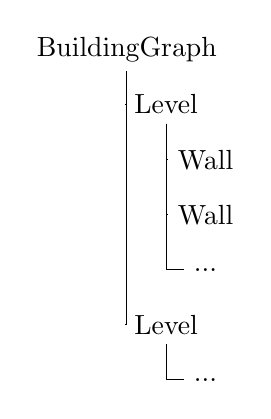
\begin{tikzpicture}[%
  grow via three points={one child at (0.5,-0.7) and
  two children at (0.5,-0.7) and (0.5,-1.4)},
  edge from parent path={(\tikzparentnode.south) |- (\tikzchildnode.west)}]
  \node {BuildingGraph}
    child { node {Level}
        child { node {Wall} }
        child { node {Wall} }
        child { node {...} }
    }		
    child [missing] {}
    child [missing] {}
    child [missing] {}
    child { node {Level} 
    child { node {...} } };		
\end{tikzpicture}
\end{figure}

The graph representation allows for some useful properties. For one thing, adding and removing walls is a simple operation on the Model. This keeps a separation from the very complex recalculation of the level geometry in the Render. We can also poll the graph for interesting properties of the Level. For example, by detecting Cycles in the level, tools could be modified to automatically generate ceilings, roofs and floors. This was not implemented in the proof-of-concept version of the software provided here to prevent feature creep. The graph model is used extensively in the geometry generation algorithm detailed in Section~\ref{sec:mesh}.

\section{Wall Rendering and Dynamic Meshes}
\label{sec:mesh}

The naive approach to rendering walls would be to create one Wall object for every wall in the graph. However, this causes visual artifacts when the walls are three dimensional. In order to solve this problem, it was necessary to construct the level mesh procedurally.

Using the graph model outlined in Section~\ref{sec:graph} as a basis, it was possible to write a custom algorithm to determine the shape of the mesh. The generator was fully encapsulated within the \verb|MeshGenerator| class; this class provides static functions which return two Mesh objects, one for rendering and one for collisions. The steps of the generation are as follows:

\begin{enumerate}
\item Generate the top-down polygon view of the Level with \verb|GenPolygons()| (described below).
\item For every edge:
\begin{enumerate}
\item Project the start and end positions up by the wall height to form two new vertices.
\item Connect two triplets of these vertices to form two triangles, which together form the face of the wall.
\end{enumerate}
\item Generate the ``tops" and ``bottoms" of each connected component as closed polygons.
\end{enumerate}

The operation of GenPolygons is as follows:
\begin{algorithm}[h]
\LinesNumbered 

\TitleOfAlgo{GenPolygons}
\KwData{A set $W$ of walls and $E$ of Endpoints.}
\KwResult{A set $P$ of polygons (vertex lists).}

Initialise $P := \emptyset$.

For every $e \in E$, construct a \textbf{clockwise ordered} list of incident walls $W_e$.

For every $e \in E$, initialise a ``visited" list, $V_e = W_e \times \{false\}$.

\While{there exists an endpoint $e$ which is unvisited from an incident wall $w$}{

Start a new empty polygon in P.

\Repeat{e is reached again}{
Set $V_e(w) := true$\;

Add a new vertex to the current polygon, $p$. If the junction is singular (i.e. the end of a wall with no connecting walls), the vertex will be exactly $wallThickness / 2$ away from the wall. Otherwise it will be at a distance dependent on the two incident walls to that vertex (see Section~\ref{sec:meeting}).

Set $e$ to the ``next" vertex. This will be the ``other" end of the next wall, or if the junction is singular it will be the other side of the same wall.
}

}
\end{algorithm}

The GenPolygons algorithm relies on a few tricks of traversing graphs. One is that the total number of times each vertex must be visited to capture every edge is equal to the number of edges incident to that vertex. In fact, the algorithm stores \textit{two} Visited lists per vertex, one for entering and one for exiting, from each edge. In this way it is possible to ensure that both sides of every wall are covered. The algorithm is able to handle cycles in the graph (i.e. enclosed rooms), as the inside and outside are treated as different polygons. Polygons are traced clockwise, except for fully internal cycles which are traced counterclockwise, by the nature of the algorithm. The order itself does not affect rendering. 

\subsection{Incident walls}
\label{sec:meeting}
The GenPolygons() algorithm uses some decisions that were made during the Design step. In particular, the walls were designed to be the same thickness throughout and should be angular rather than rounded. It was decided that when two walls were to meet at a corner, rather than mitre the edge (cut or round off the sharp corner), it should be ``sharp". See the figure for a couple of examples. A number of different ways of constructing this were tried. In the end the method used was to project the ``inside" vectors of both walls and calculate the point on the plane where they meet, and do the same for the ``outside" reflexive angles. This produces ideal results in the vast majority of cases, though walls do protrude a long distance when they meet at very sharp angles. 

Constructing the edge list on each vertex and handling the meetings pairwise means that the algorithm can handle arbitrarily many walls meeting at one point. However there are some cases it is not designed to handle, such as when two walls overlap but do not meet at any junctions. It would be possible to handle this case in a number of ways: to disallow the tool from creating such walls; to create a junction at the intersection point; or to only build the wall up to the point where it intersects with an existing wall. The proof of concept tool does not distinguish this case.

\subsection{Results}
Employing this algorithm removed all cases of overlapping textures and depth fighting arising from two wall textures meeting. On very sharp angles, the distance travelled by the 
Preliminary testing showed that the algorithm ran well within one frame (approximately 11ms) on reasonably sized levels. There was little to no slowdown even on more difficult cases, such as many complete polygons and endpoints with a large number of incident walls\textsuperscript{F5}. 


\section{Doorways and Constructive Solid Geometry}
\label{sec:csg}

The wall mesh outlined in Section~\ref{sec:mesh} is extensive and produces high quality output, but it only produces flat vertical faces. In order to replicate architecture in a realistic manner, it is necessary to cut holes in the walls, for doors and windows. The technique employed here is called \acrlong{csg}. A special case of the \acrshort{csg} technique is used to deal with our non-primitive, pre-defined wall mesh.

\subsection{Theory}

\acrlong{csg} is an extension of the 2D technique known as Boolean Operations on Polygons. This system relates the traditional boolean operations (AND, OR, XOR) and binary subtraction, to geometric shapes. For example, \verb|Union()| on two overlapping squares will create a polygon from the outer perimeter of the two. The CSG and BOoP systems are both used in many \acrlong{cad} programs, as they can be used to model complex systems and shapes with very simple definitions. The algorithms backing both CSGs and BOoP are complex and have only been implemented a handful of times across all platforms. The most notable implementation is CGAL~\cite{cgal},  which is a collection of a large number of 2D and 3D geometric algorithms in C++. There is no known best time complexity for CSG in the general case, but \cite{csgsub} has an upper bound of $n^4$ where $n$ is the number of primitive faces. It is unrealistic to calculate CSGs every frame for our application which may have a large number of subtractions.


\subsection{Implementation}
\label{sec:csgimp}

The usage of CSG for this application was a very restricted case. We only needed to: [a] cut holes (subtraction operation); [b] with cuboids, from cuboids; [c] which were axis aligned relative to each other. In this case it was suspected that the algorithm could be implemented directly without resorting to complete CSG; this would also greatly improve the runtime complexity. The initial implementation plan was to go ``along" each wall, drawing full-height quadrilaterals where there were no holes and partial-height quadrilaterals around the top and bottom of holes. This would have worked well. However, the algorithm would not succeed on the far more complex wall meshes which were designed by the algorithm in Section~\ref{sec:mesh}; junctions can be constructed such that one side of a wall is much longer than the other side, which would make computing the correct vertex locations very difficult.

As a result, it was decided to fall back on a full CSG library. The technique here would be to create cuboid objects in the relevant locations and use the \verb|Subtraction| operation to ``cut" the holes from the main LevelRender mesh. After exploring the options we settled on the CSG library known as \verb|CSG.cs|~\cite{csgcs}; This is a port of the popular Javascript library \verb|CSG.js|~\cite{csgjs} to the C\# language, with specific Unity bindings. It is designed such that the programmer can provide two Unity objects (in our case the \verb|LevelRender| mesh and the \verb|Hole| cuboid) as parameters to the relevant binary operation (here, \verb|Subtraction|).

In order to improve expected run times, all Holes in the Level were first collected with the Union operation into one mesh composed of many constituent cuboids. This meant that only one Subtraction operation needed to take place, and the Bounds and Normals of the mesh need only be recalculated at the end. 

\subsection{Intelligent Placement}

Placing multiple Holes overlapping would be likely to cause the CSG operation to take longer; it may also create artifacts, which would be an undesirable outcome for the architect. As a result, an intelligent placement system was embedded in the Doorway/Window tool. Given the length of the Wall and the current number of Holes in it and their positions, it is possible to calculate whether or not a new Hole is in a valid location ahead of time and before the expensive CSG operation. When the position is invalid, the Wireframe outline turns red and the tool disallows placement of the Hole.

\subsection{Results}

The results for implementation were positive and negative. The CSG implementation correctly cuts doorway and window holes as expected. However there are some downsides to using the full CSG library. For one thing, the subtraction operation is slow. It was possible to reduce the runtime by approximately 50\% with the improvements described in \ref{sec:csgimp} but there was still significant slowdown with more than 20 holes on one level. This issue is mitigated by some of the features of SteamVR; see Section~\ref{lag} for more information. An upside of the system design is that only the current horizontal Level is updated when the geometry is changed; as a result a world with 100 doorways on the ground floor will still see fast updates on the first floor.

A benefit of using full CSG methods is that it is theoretically possible to create arbitrarily shaped holes, including archways or circular windows. These were avoided in this project, as it was suspected that introducing more complex geometry would significantly increase the run time of the CSG operations. At present, the CSG system does not correctly modify the collision mesh used for doorways as the result of an issue with two-dimensional meshes. This means that it is not possible to target a point ``through" a doorway with the current implementation.

Despite its failings, the CSG library does show its power --- using only two or three commands it is possible to create and modify almost arbitrary shapes. Better optimised CSG libraries, including the ones in CGAL, may be able to provide a more appropriate feature set, or perform the same operations with improved run times.

\section{Lighting Model}
\label{sec:lighting}

By default, Unity uses a combination of different lighting and shading models. For specular shading (on objects which use the ``Default (specular)" shader), BlinnPhong illumination is used; For diffuse shading, the Lambert lighting model is used. It is possible to change the lighting model to a different algorithm and include custom shading models~\cite{customlighting}; this was considered to be out of scope. 

The lighting in the software is provided from three different sources.

\subsection{Global Illumination}
\label{sec:gi}

Almost all lighting in the World is provided by \acrfull{gi}. Unity relies on GI to emulate complex indirect lighting very efficiently. Realtime Global Illumination is achieved in Unity by carefully pre-computing (\textit{baking}) all possible lighting situations and how light would bounce. This is only available for static objects however, and so the software can only use these for the Principal objects (see Section \ref{sec:principal}). 

In cases where full GI cannot be achieved at runtime, Unity falls back on Ambient lighting - a base amount of light which exists in all places and is used to light objects which would otherwise be in total darkness. Our software uses a fairly high Ambient lighting level; this means users can see and work on rooms which would be very dark in reality. 

\subsection{Directional Lighting}
\label{dir}

By default there is one main directional lighting source in the World: the Sun. Using the Weather tool it is possible to change not only the position of the Sun, but the colour and intensity of the light that it provides. Shadow is cast by everything in the World, including walls, floors, ceilings and objects. Because the shadow cast is dependent on the rendered mesh, cutout doorways and windows do not cast shadows (as is expected). 

\subsection{Point Light Sources}
\label{sec:points}

One of the Objects provided with the software is a Lamp; when this lamp is placed, a Point light source is attached to it such that it gives out a small amount of light. Due to the partial lighting computation, there were originally some minor artifacts with walls. However, being able to customise the lighting of a building is an important part of architectural design. The introduction of three-dimensional walls removed the problem of light bleeding through to other rooms.


\section{Roofs and Straight Skeletons}
\label{sec:roof}



\section{Interaction in VR}
\label{sec:interaction}

\section{Importing Objects}
\label{sec:objects}
\label{sec:import}
The system was designed to allow the users to easily import their own furniture and other kind of objects into the program. The system itself contains no hard-coded objects that can be placed in the scene. Instead the user can place specially created Model files in the \verb|main_Data\AssetBundles| directory in the installation location. When this is done, the program will import them  at runtime. This is implemented using Unity's AssetBundles~\cite{unity:assetbundle}. These are designed exactly for the purpose of storing Unity assets in a format that can be loaded by the application at run time. The ability to load in assets without recompiling the program makes it more flexible, versatile and dynamic\textsuperscript{F3}.

In order to supply users with initial set of objects, a special button was added to the editor under the Assets menu to allow for a creation of a basic set of objects to be used within the game.

\section{Saving and loading a scene}
\label{sec:saving}
To allow the user to save and load the projects they have been working on, a save and load menu was implemented\textsuperscript{F6}. This has been achieved using the Serialisation method~\cite{unity:serialization}. The separation of model from view was used in this process as native Unity classes are not possible to serialise, which meant that only the underlying models were possible to easily serialise and write to a file. During the loading phase the models have to be replaced by the ones found in the file, and Unity-specific objects need to be reconstructed from that model. The serialisation process creates a new file that is independent from the rest of the project. These serialised files can be transferred between different machines by copying the produced \verb|.sav| files between the \verb|projects| directories on different machines\textsuperscript{NF3}.

\section{Unity features in use}
Apart from the previously mentioned AssetBundles~\cite{unity:assetbundle} and the serialisation method~\cite{unity:serialization}, a number of other Unity methods were used to speed up the development process. An important feature here is the in-built ray casting in Unity that is used in all the tools to determine the object or the location the user is pointing at. A related feature to this are the layers, which allowed certain objects to be excluded when performing ray casting; this was mainly used in the Paint Floor tool to ignore the Blueprint object which was located above the floor segment and perform ray casting against floor segments only. Without the layers the ray casting would collide with the blueprint object (which was closer to the user) instead of the floor segments.

Unity's prefabs are used to store the objects that can be placed in the scene. The prefabs that are stored in the asset bundle are used to instantiate new Unity objects as a duplicate of the original object.

Another useful feature of Unity that was used in this project was Unity's support for distributing assets. The editor has an inbuilt range of Standard Assets, some of which were imported into the project. Unity also has its own assets store, which allows developers to download third-party assets (including scripts, 3d models and textures) into their project for free or for a small charge.

% Expand on what Standart Aseets we used?

\section{Imported Assets}
In order to spend time working on the system rather than dynamic content, a number of external 3D models were used in the program. Two packages were acquired from the Unity Asset Store and are provided with the project as a proof of concept. Those packages are:
\begin{itemize}
    \item \textbf{Free Furniture Set} - a collection of wooden furniture, available at\\ \url{https://www.assetstore.unity3d.com/en/#!/content/26678}
    \item \textbf{Gray Furniture Pack} - a collection of grey furniture and electronics, available at \url{https://www.assetstore.unity3d.com/en/#!/content/40580} 
\end{itemize}

Those assets are available free of charge and the licensing allows them to be used in our project as discussed in section~\ref{sec:legal}.

%\chapter{User Guide}
%\label{chp:user_guide}
%\section*{Installing Unity}
To run or build the provided source code two things need to be installed on the system:

\begin{enumerate}
    \item Unity - the editor in which the provided code can be opened. To install follow the instructions at \url{https://docs.unity3d.com/Manual/InstallingUnity.html} % Need to check if it will work with any version
    \item Steam \acrshort{vr} - a library that provides \acrshort{vr} support for the project. To install it, Steam must be installed first before Steam \acrshort{vr} can be installed: \url{http://store.steampowered.com/steamvr}
\end{enumerate}

After the above components are installed on the system, the provided source code can be opened in the Unity editor. After opening it in the Unity editor, the furniture assets need to be prepared in order for the Object Tool to work as intended. To do this click Assets > Build AssetBundles from the menu bar. Only then the project can be run on the local computer.

\section*{Installing the project}
To build the project with Unity select File > Build Settings... This will open a new window in which you can specify some build details. Click Build to build the project as a standalone piece of software in the specified location. To supply the build project with default furniture assets, copy \verb|AssetBundles\sample| file from the source code and copy it into \verb|main_Data\AssetBundles| directory in the build location. The program can then be execute by running the newly created executable main file.

\section*{Using the program}
The following section will describe different parts of using the application. The image will figure~\ref{fig:vive_controllers} will be used as a reference to explain what button to press when using the program.

\begin{figure}[!ht]
 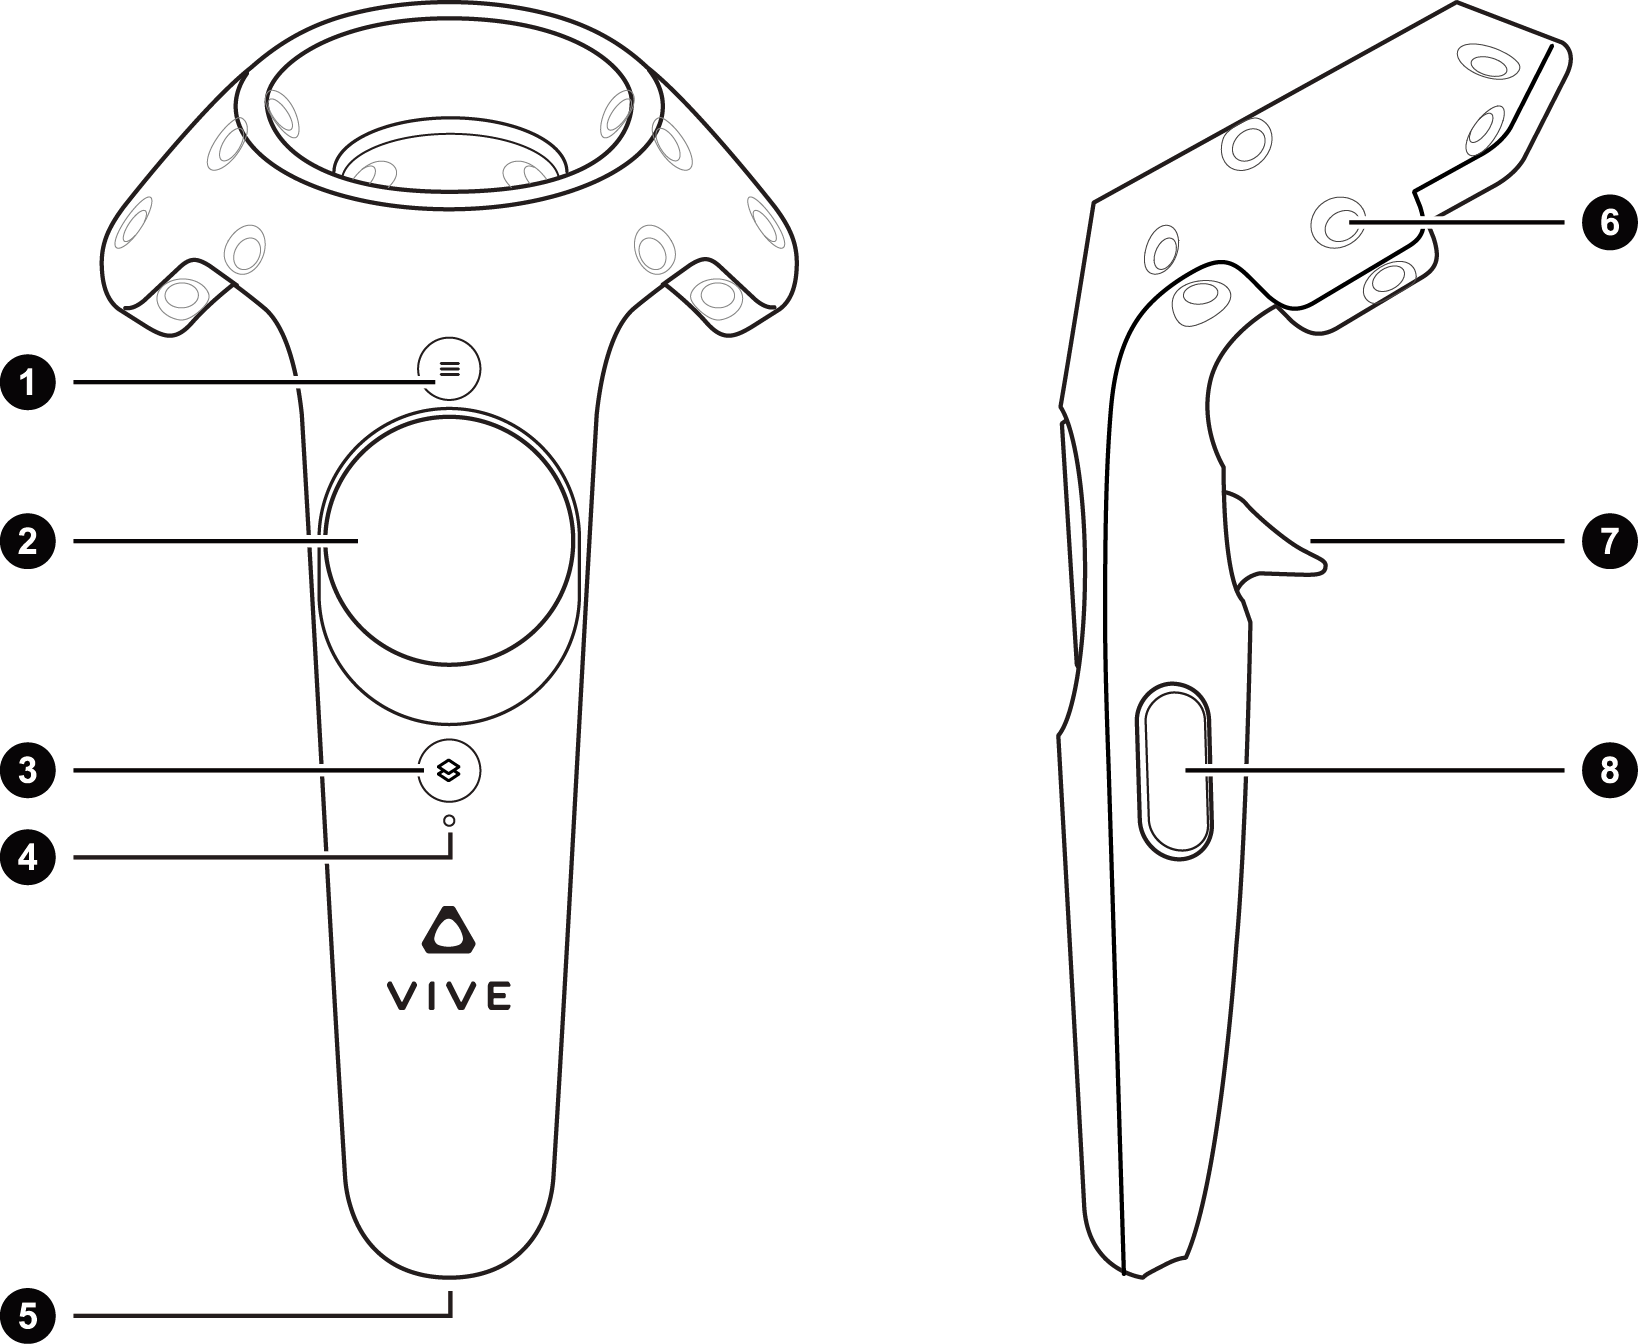
\includegraphics[width=\textwidth]{ViveControllers}
 \caption{HTC Vive controllers}
 \label{fig:vive_controllers}
 % Taken from https://docs.unity3d.com/Manual/OpenVRControllers.html but can't find a good reference for it
\end{figure}

% TODO: ??? need to  be replaced with the relevant VR button 

\subsection*{Changing tools}
To change the currently used tool, a tool menu has to be opened first. This can be done by pressing ???, which will toggle the menu between the open and closed state. Closing and opening the menu again will always reopen it directly in front of the user. The tools can then be selected by pointing at the icon representing the desired icon and pressing ??? with the controller that should become that tool.

\subsection*{Saving and loading previous projects}
Saving and loading previous projects can be done via an additional menu which can be opened and closed by pressing ???. Similarly to the tool menu, it will always be opened directly in front of the user.

\subsection*{Example}
The example below will lead you through the process of creating a basic room and saving your progress:
\begin{enumerate}
    \item Move to the place where you want to start building your room by either physically walking over to that location or using the teleport tool. To use the teleport open the tool menu by pressing ??? and select a teleport tool by pointing at it with the laser and pressing ??? on the controller. The controller on which the ??? was pressed will be the controller that the teleport tool is assigned to and it'll be the controller that will be used to teleport.
    \item Change the tool to wall tool and use it to build 4 walls of your room forming a rectangle. If you closed the menu, or walked far away from it you can close it and reopen it by pressing ???. To build a wall point at the place you want it to start from and press and hold ???. Then point to the location where you want the wall to end and release the presses button. If you started the wall in the wrong place point at the sky to cancel that wall segment. The line drawn on the ground shows where the wall is going to be places, so you can see if it starts and ends in the desired location.
    \item Select the floor build tool from the tool menu. Press ??? to select 4 points on the ground that match up with the corners of your room. If you misplaced one of the points you can press ??? to cancel the last point. When the 4 points are places press ??? to confirm and create a new floor segment. The lines drawn show you where the floor you are creating now is going to be placed.
    \item To paint the floor, change to tool o the paint floor tool and point at the floor you want to paint. Press ??? to toggle between the textures and ??? to apply the texture to the floor that is being pointed at. The same tool can be used to apply different textures to objects as well.
    \item To add objects to the scene select the add object tool. The green ghost object will show you where the object is going to be places. You can rotate it using ???, reset the rotation by pressing ???, change the object with ??? and confirm the placement with ???. The objects can be stacked on top of each other and can be automatically rotated to perpendicular position to the surface you're pointing at with ??? (for example making perpendicular to the wall rather than the floor).
    \item To add a doorway select the add doorway tool. To place a doorway point at the place in the wall where you want the doorway to be places and press ???. Once placed doorway cannot be removed and multiple doorways can be joined together to create a wider passage. To place a door use the add object tool.
    \item To add a ceiling change the floor level to one above the current one using ??? and create a floor with a floor build tool that corresponds to the area you want to be covered by the ceiling in the floor below. You can then use the floor painting tool to change the texture of the ceiling. You can then go back to the original floor by pressing ???; Alternatively if you are not planing on building future floor above, you can build a roof instead of a floor segment using the roof building tool.
    \item To save the current project bring up the save/load menu by pressing ??? and select the save option from it with either controller by pointing at it and pressing ???.
    \item Exit the program and bring up the save/load menu. Press the load icon corresponding to your project by pointing at it with a controller and pressing ???.
\end{enumerate}

\chapter{Testing}
\label{chp:testing}
The software we have built is a product designed for use by many different people in a range of environments. There are many complex algorithms which interact with each other, which may be prone to bugs. Working in a VR environment provides additional quality assurance concerns, such as user comfort and intuitive design. As a result, our testing strategy formed an important part of development. 

\section{Systems and Integration Testing}

Each new feature that was added underwent a rigorous set of tests to ensure that it operated correctly in all cases. This was a qualitative process, though rather than simply using the new features, test cases were chosen specifically such that they would prove correctness in unusual situations and fringe cases. Some of the more extreme tests, such as the stress testing of wall mesh generation, became Unit tests and were repeated at later instances to ensure functionality had not been lost.

A good example of where integration testing was useful was with the Tools menu. When dealing with new tools such as Object placement and Selection and Floor construction, we found that the Tools menu could not be interacted with, meaning the user could not use the menu - in fact, the user placed objects onto the tools menu or drew a floor vertex on it, respectively. These tools were then modified such that they could not target the tools menu, and when they did they changed tool rather than activating. These issues would not have been discovered with piecemeal system testing, and only through immersive integration testing were they found.

All opportunities were taken to test new systems in the VR environment as well as on the Desktop. This was difficult due to the overheads of time and effort required in setup. In times where this was not possible, VR could be emulated on the destkop by manually specifying the \verb|inputMode| as part of our \verb|InputControl| class; the Controller objects could be moved manually within the editor to simulate the user moving the real-world controllers. This method was used initially to test analog controls such as weather manipulation and object scaling, though they were later proven correct in the VR system during full Quality Assurance testing.


\section{Unit testing}

Not all systems were appropriate for unit testing, though the more abstract systems had a number of features which could be tested. In particular the mesh generation algorithms, menus, and graph model could be inspected for correctness. Unit testing was repeated during each QA testing period to ensure that no bugs had been introduced with the addition of new features, and additional unit tests were written to test any new features. Unit tests were performed by hand and not automated due to the nature of the software. Please see Table~\ref{tab:unit-tests} for the final set of unit tests, all of which the software passed.

\section{Quality Assurance Testing}

Our initial project roadmap (see Section~\ref{sec:timetable}) set aside four periods of time dedicated to QA testing; these were around Weeks 9, 14, 20 and 28. The longest of these was the third, which covered weeks 20 to 22 inclusive. Having large periods of time devoted primarily to Quality Assurance meant that we were able to make minor changes to the operation of the software without introducing any new systems in the meantime. In this way, we could ensure that most bugs were removed prior to moving on and adding new, large feature sets. The last period of QA took place after the feature freeze starting in Week 26 (during the Easter holiday), and was alongside the main bug fixing session. This allowed us the freedom to add more ``polish" to the final product without worrying about introducing more issues along the way.

An additional note about QA testing in room-scale VR is that it requires more commitment than QA testing for a normal application. This is the result of a number of factors. For one, some people simply do not like the Virtual Reality environment, so finding people to test the application is more difficult. Another concern is that we were explicitly testing for intuitive usage (Non-Functional requirement 1); we found that when people became used to the VR environment after the first try with the software, they were not able to determine whether or not the controls were intuitive. 

Our approach to QA testing was qualitative rather than quantitative. Our pool of testers primarily comprised peers in the Department of Computer Science, as well as members of the University of Warwick Game Design Society. These testers were chosen both for willingness to engage with the software and their relative objectivity, but also because it was expected that they could provide useful and actionable feedback. Our testers spent around ten minutes using the software. During this time we took into account several factors, such as what they were doing within the World, how they interacted with menus and objects, and whether or not they were effective in their usage. We also noted any comments they made during this time. The time using the software was limited to ten minutes to reduce the risk of nausea and eye strain.

There are also physical requirements which can only be tested when the software is exposed to a range of people. One example is that in the Desktop version of the tool, the user's head height is fixed at 1.5m above the current floor level. Things such as doorways, windows and objects are designed around this. As a result, particularly short or tall people may have vastly different experiences with the tool. After testing we were able to mitigate some of these issues, such as by allowing the user to position the Tool and Save menus themselves. Doorways and window heights were modelled on their real world counterparts.

After the testers had completed their session, they were asked to describe their experience in the abstract. We found that asking this first gave a wider range of answers. After this, we asked more specifically about different aspects of the software, with questions like:

\begin{itemize}
    \item ``Did you enjoy using the software?"
    \item ``Did you find that there was any lag or stuttering during your time with the software?"\textsuperscript{F5}
    \item ``Was the software intuitive to use? Were there any tools which you had trouble using?"\textsuperscript{NF1}
    \item ``Did you notice any visual artifacts or glitches with the architecture"\textsuperscript{F1,F4}
\end{itemize}

This gave us direct feedback on our progress with respect to the original requirements analysis. By the fourth QA testing period, we were receiving positive feedback in general and on the specific questions outlined above. This gave us a positive indicator that our software was meeting the functional and non-functional requirements we had laid out.

In order to test the long-term effects of using the tool, as well as assessing the performance on larger buildings, the project team tested for longer periods of time. All team members reported that they were able to comfortably use the software for more than 30 minutes with no ill effects. One team member reported minor eye strain; this is attributed to not being able to wear larger models of glasses when in the \acrshort{hmd}.

\begin{table}[]

\centering
\caption{Final set of Unit Tests used during QA4}
\label{tab:unit-tests}
\begin{tabular}{lp{10cm}c}
\hline
\textbf{Testing Group}             & \textbf{Test}                                                                                          & \textbf{Result} \\ \hline
\textbf{(1) Wall mesh}             &                                                                                                        &        \\
\textbf{}                          & Wall placed from point A to B is spawned from A to B\textsuperscript{F3}                               & \ding{51}       \\
\textbf{}                          & Walls placed are correct width                                                                         & \ding{51}       \\
                                   & Graph with 100 edges generates mesh in \textless 11 ms\textsuperscript{NF1}                            & \ding{51}       \\ \hline
\textbf{(2) Wall correctness} &                                                                                                        &      \\
                                   & 90 degree corner generated correctly                                                                   & \ding{51}       \\
                                   & T-junction generated correctly                                                                         & \ding{51}       \\
                                   & Box (closed loop) of walls generated correctly                                                         & \ding{51}       \\
                                   & 16 pointed star (one junction) generated correctly                                                     & \ding{51}       \\
                                   & Walls of length 0 not generated                                                                        & \ding{51}       \\
                                   & Walls which overlap not generated                                                                      & \ding{51}       \\
                                   & Wall meshes placed at correct position on Y axis                                                       & \ding{51}       \\ \hline
\textbf{(3) Roof mesh}             &                                                                                                        &        \\
                                   & Roof mesh is spawned at correct position on Y axis                                                     & \ding{51}       \\
                                   & Triangular, rectangular, octagonal roofs genrated correctly                                            & \ding{51}       \\ \hline
\textbf{(4) Floor mesh}            &                                                                                                        &       \\
                                   & Floor mesh is spawned at correct position on Y axis                                                    & \ding{51}       \\
                                   & Triangular, rectangular, octagonal floors genrated correctly                                           & \ding{51}       \\ \hline
\textbf{(5) Painting}              &                                                                                                        &        \\
                                   & Walls, floors, roofs, and objects can be painted\textsuperscript{F3}                                   & \ding{51}       \\ \hline
\textbf{(6) Deletion}              &                                                                                                        &      \\
                                   & Floors, roofs, and objects can be deleted\textsuperscript{F3}                                          & \ding{51}       \\ \hline
\textbf{(7) Objects}               &                                                                                                        &        \\
                                   & Objects can be selected with the Selection tool                                                        & \ding{51}       \\
                                   & Objects are placed at the rotation of the controller                                                   & \ding{51}       \\
                                   & Objects can be scaled                                                                                  & \ding{51}       \\ \hline
\textbf{(8) Weather}               &                                                                                                        &        \\
                                   & Time of day can be changed                                                                             & \ding{51}       \\
                                   & Lighting channels can be changed on the Sun                                                            & \ding{51}       \\ \hline
\textbf{(9) Menus}                 &                                                                                                        &       \\
                                   & Tools and Save menus are summoned on button press\textsuperscript{F2}                                  & \ding{51}       \\
                                   & Tools and Save menus are un-summoned on button press                                                   & \ding{51}       \\
                                   & The menus can be used with any tool selected\textsuperscript{F2}                                       & \ding{51}       \\ \hline
\textbf{(10) Saving/Loading}       &                                                                                                        &       \\
                                   & Pressing the Save button creates a correct save file\textsuperscript{NF3}                              & \ding{51}       \\
                                   & Pressing the Load button for a save file loads the file as it was before saving\textsuperscript{NF3}   & \ding{51}       \\\hline    
\end{tabular}
\end{table}

\section{Testing Against the Specification}

As mentioned in the specification section of this report, throughout this section the use of a superscript requirement code (like this\textsuperscript{F3}) is done to demonstrate that the passing of the given test indicates that the associated requirement has been satisfied in full.

\chapter{Project Management}
\label{chp:project_management}
When undertaking any project, several challenges may come to light and subsequently must be rigorously accounted for with appropriate documentation during the planning, design, and implementation phases of the project. Some of these challenges could be the organisation of the team members, the selection of what tools that team members shall use, or the software development methodology itself. The purpose of this chapter is to discuss areas of project management such as these, and how the group and its members overcame challenges like them throughout the project's life cycle.

\section{Project Methodology}

    \subsection{Project Summary}        
    
        To gain a clear understanding of any software development project, a few key tasks must be first complete before any development work can be done. The project aims and resources to achieve them must be clearly defined, and the stakeholders in the project should be identified. Once these steps have been taken, it's also crucial to justify the project to each group member as to ensure that they are individually happy with why and how the project will move forward. For this project this has already been discussed in detail within chapter~\ref{chp:specification}, though this section will contain a summary of this specification from the perspective of project management.
        
        The original project idea was proposed and accepted with intrigue and excitement from all group members after an initial enquiry into its feasibility, given that the hardware to test virtual reality software is not common place. Once this concern was addressed with the Computing Society at the university giving the group access to the HTC Vive \acrshort{vr} system. The project gave the group members an opportunity both to work with a novel \acrshort{hci} technology, and to work on the cutting edge of the research into possible industrial uses of \acrshort{vr}. Using the HTC Vive, the group set out with the objective of creating a tool that can be used to aid the architectural design and visualisation process, allowing the user to create and manipulate 3 dimensional spaces in a virtual reality.
        
        With a large project scope, it was decided to develop the software as a proof-of-concept with a minimal list of tools that provided all of the functionality necessary to meet the project objectives and aims. With the project's approval by its supervisors, the following work consisted of determining a use case to work toward, researching \acrshortpl{sdk} and best practises for developing a virtual reality application, and finalising the list of basic tools to be implemented in the project software. Once these tasks were completed, a list of common household items to be included as assets was drawn up. As described in section~\ref{sec:progress_management}, the progress of the project's stages was monitored, with the tasks being scheduled between members both evenly and to suit each member's individual strengths where possible. The project was tested frequently to also monitor potential software problems and functionality regressions as time went on. In the final stages of the project, the departmental project deliverables were consolidated and brought to a conclusion to ensure that it is delivered safely whilst also addressing the project's previously established objectives.

    \subsection{Software Development Methodology}
    
        As with any software development project, it is necessary to consider enacting an appropriate development methodology. If not, the lack of effective practices can lead to unpredictable functionality, poor code quality and documentation, and repeated error. Software development methodologies range from the rigid-structure, document centric waterfall approach to more agile methods that prioritise adaptability to requirement changes and code quality. With a small project group size of just 3 people who have fluctuating schedules week-upon-week and thus time that can be dedicated to project work, a variation of the scrum agile methodology was chosen. Core concepts of an agile methodology were retained like the frequent delivery of working software, welcoming continuous changes in requirements, and daily cooperation between developers~\cite{martin2003agile}. Other methods such like waterfall were considered inappropriate within the context of this project due to their inflexibility with changing requirements, or for being geared toward more enterprise-like group sizes where teams can be 10s to 100s of developers in size.
        
        With the flexibility of development introduced by the an agile methodology, internal milestones for software development were put in place with the flexibility to cater for changes in requirements. The group structure also reduced the focus on sprint-based development that lies within traditional scrum-based methods due to there being no emphasis on delivering functional products to the project stakeholders on a regular basis. The group structure consists of one development team of 3 individuals, opting to replace frequent (typically daily) scrum periods with sporadic development sprints that are encapsulated by discussion between development team members.
        
        With some parts of the project being independent from others, it was possible to use the scrum methodology effectively to allow two members to complete these tasks simultaneously. Because of this, any iterations upon these independent tasks was also possible without as much planning as would be necessary if they were dependent, helping the fact that the project has a small time frame. Frequent meetings with project supervisors generated feedback that could be acted upon within a short time frame thanks to the agile method that was adopted. It is also important to recognise that the agile method does carry the danger that sufficient documentation of a code base will not be created, thanks to its code-centric approach to development. This affects teams that have members that are constantly in flux. Fixed teams that do not change are unlikely to run into this problem, though it should be made imperative that documentation is monitored to avoid the documentation becoming stale.
        
\section{Team Structure}

    As mentioned in previous sections of this report, the project group consists of 3 members, originally starting with 4. With such a small group of people, it was imperative that the work load was balanced as equally as possible. With the loss of a group member at an early stage in the project, it was also necessary that task distribution was also done intelligently to account for the loss in expertise. Work was also divided in a way to play to each member's individual strengths. With 3 group members it was impractical to try split work between at least two people, but a focus on clear and concise documentation meant that if a group member had to fill in for another, they could swiftly get up to speed with the work. Whilst there are obvious benefits to having a larger number of people in a group, there are also benefits to small groups; organisation is simpler, the allocation of tasks is straightforward, and each group member is more aware of the work they have been assigned. A smaller group does leave a disadvantage when it comes to the sheer number of developers available to work on the project at any one moment. The individual members of this project and their assigned roles are shown below:
    
    \begin{itemize}
        \item \textbf{Alex Dixon - Mesh generation, UI, and software back end architect.} Responsible for the primary mesh generation algorithms for walls, floors and roofs, the user interface, and the abstract representation that is used to generate the meshes.
        \item \textbf{David Richardson - Project manager and environment manipulation.} Responsible for the distribution of tasks between group members and managing deadlines, as well as the implementation of environment lighting manipulation functionality.
        \item \textbf{Jakub Zawadzki - Tools developer and 3D asset builder.} Responsible for the architecture of the tool subsystems and the construction and exporting of 3D assets for inclusion with the final software deliverable.
    \end{itemize}
    
    Whilst this list is not exhaustive, it serves as a good demonstration of the group's ability to allocate tasks to each member and for them to take responsibility for them.

\section{Time \& Task Management}
\label{sec:timetable}

    The effective management of the time allocated to a project is necessary to ensure it is completed within the given time constraints. Because of this it is necessary that tasks are identified and scheduled for completion in an appropriate time frame. Figure~\ref{fig:project_timetable} gives a Gantt chart that gives an outline of the task break down of the project, the scheduling of those tasks, any inter-task dependencies, and important internal milestones for the group throughout the lifecycle of the project.
    
    \begin{sidewaysfigure}
		\centering
		\begin{ganttchart}[
			x unit=5.25mm,
			hgrid,
			vgrid,
			newline shortcut=true,
			time slot format=simple,
			bar/.append style={fill=Aquamarine!25},
			bar label node/.append style={align=right},
			milestone inline label node/.append style={right=3mm},
			milestone/.append style={fill=RubineRed!50},
			today=30,
			today rule/.style= {red, ultra thick, dashed},
			today label={Product delivery},
			link bulge=.5,
			link/.append style={thick}
		]{1}{31}
			\gantttitle{Term 1}{10}
			\gantttitle{Christmas}{4}
			\gantttitle{Term 2}{10}
			\gantttitle{Easter}{5}
			\gantttitle{Term 3}{2} \\
			\gantttitle{Time (in weeks)}{31} \\
			\gantttitlelist{1,...,31}{1} \\
			\ganttbar[name=feasibility]{Feasibility study}{1}{2} \ganttmilestone[inline=true]{First prototype}{7} \ganttmilestone[inline=true]{Final prototype}{20} \ganttnewline
			\ganttbar[name=concept]{Concept design}{3}{4} \ganttmilestone[inline=true]{Second prototype}{10} \ganttmilestone[inline=true]{Feature freeze}{25} \ganttnewline
			\ganttbar[name=uidesign]{UI development}{6}{8} \ganttbar[name=uidesign2]{}{11}{13} \ganttbar[name=uidesign3]{}{23}{24} \ganttnewline
			\ganttbar[name=qa]{Quality assurance}{9}{10} \ganttbar[name=qa2]{}{14}{15} \ganttbar[name=qa3]{}{20}{22} \ganttbar[name=qa4]{}{27}{29} \ganttnewline
			\ganttbar[name=sysdev]{Systems development}{6}{9} \ganttbar[name=sysdev2]{}{12}{15} \ganttbar[name=sysdev3]{}{18}{19}
			\ganttnewline
			\ganttbar[name=assets]{UI development}{16}{17}
			\ganttnewline
			\ganttbar[name=bugfixes]{Bug fixing}{25}{29}
			\ganttlink{feasibility}{concept}
			\ganttlink{concept}{sysdev}
			\ganttlink{concept}{uidesign}
			\ganttlink{sysdev}{sysdev2}
			\ganttlink{uidesign}{qa}
			\ganttlink{qa}{uidesign2}
			\ganttlink{uidesign2}{qa2}
			\ganttlink{qa}{sysdev2}
			\ganttlink{qa2}{sysdev3}
			\ganttlink{qa3}{uidesign3}
			\ganttlink{uidesign3}{bugfixes}
			\ganttlink{sysdev2}{sysdev3}
			\ganttlink{sysdev3}{bugfixes}
			\ganttlink{sysdev3}{qa3}
		\end{ganttchart}
		\caption{Project timetable from week 1 term 1 to week 2 term 3}
		\label{fig:project_timetable}		
	\end{sidewaysfigure}
	
	Along with the development of the software for the project, its deliverables also require scheduling to make certain that they are delivered on time without error. Figure~\ref{fig:document_timetable} shows the timetable breakdown of work toward these deliverables up to the point of hand in for this report.
		
	\begin{sidewaysfigure}
	    \centering
	    \begin{ganttchart}[
			x unit=5.25mm,
			hgrid,
			vgrid,
			newline shortcut=true,
			time slot format=simple,
			bar/.append style={fill=Aquamarine!25},
			bar label node/.append style={align=right},
			milestone inline label node/.append style={right=3mm},
			milestone/.append style={fill=RubineRed!50},
			today=30,
			today rule/.style= {red, ultra thick, dashed},
			today label={Product delivery},
			link bulge=.5,
			link/.append style={thick}
		]{1}{31}
	        \gantttitle{Term 1}{10}
			\gantttitle{Christmas}{4}
			\gantttitle{Term 2}{10}
			\gantttitle{Easter}{5}
			\gantttitle{Term 3}{2} \\
			\gantttitle{Time (in weeks)}{31} \\
			\gantttitlelist{1,...,31}{1} \\
			\ganttbar[name=spec]{Specification}{2}{3} \ganttmilestone[inline=true]{Specification hand in}{4} \ganttnewline
			\ganttbar[name=progress]{Progress presentation}{8}{9} \ganttmilestone[inline=true]{Progress presentation hand in}{10} \ganttnewline
			\ganttbar[name=finalreport]{Final report}{23}{30} 
	    \end{ganttchart}
	    \caption{Documentation timetable from week 1 term 1 to week 2 term 3}
	    \label{fig:document_timetable}
	\end{sidewaysfigure}
		
\section{Progress Management}
\label{sec:progress_management}

    \subsection{Meetings}
    
        Regular meetings were scheduled between the project group and supervisors every fortnight. These meetings were used to update the project supervisors on the progress of development, any successes, changes to the projects requirements, and any challenges that the group has faced recently to get advice on how to tackle them. Emergency meetings were also scheduled when urgent matters arose within the project, such as the loss of a group member as explained later in this chapter. Outside of office hours, contact with the project supervisors was maintained using e-mail.
        
        General group meetings were also arranged weekly to discuss project progress, identify any new or remaining tasks for the current stage of the project and assign these tasks to group members, and re-arrange or re-assign tasks to improve the timetabling of the project. Discussion between members about software design and review of new code was performed regularly to preemptively eliminate potential issues. Any research that had been done since the last meeting was also shared between group members to aid the understanding of the code base further in the event of task re-assignment. These meetings consisted of all 3 group members and would typically be performed within the departmental computer labs, where work could be demonstrated on laptops or departmental computers. Some meetings were also used to test prototype software, and as such required all group members to be present to help set up and operate the virtual reality system.
        
    \subsection{Weekly Project Review}
    
        As per the development methodology chose, at each weekly meeting a review of the project's current state was performed with respect to its timetable, as shown in the Gantt chart in figure~\ref{fig:project_timetable}. This review consisted of individual member updates as to the progress of their assigned tasks. By combining the individual progress of each member, the overall state of progress for the project could be ascertained. A list of things that are to be completed was constructed at each meeting, for completion by the next.
    
    \subsection{Internal Milestones}

        With the group meetings and weekly reviews, a number of internal milestones were set to work toward. These milestones represented a state in the project's development that meant the software met a number of the project requirements. A few of these milestones are displayed in the Gantt chart in figure~\ref{fig:project_timetable} as the prototype milestones and the feature freeze. Some of these milestones also served as a way to prevent feature and scope creep of the project by preventing the introduction of new features after a specific point in the project's life cycle.

\section{Collaboration Tools}
    \subsection{GitHub}
    
        To help with resource management for the project's source code and documentation like this report, several git repositories were created and utilised as source control. GitHub is a web-based git repository host and web front end for the git version control system. It provides a means to simplifying the git workflow through a number of easy to use tools and shortcuts, aiding with tasks such as the merging of code changes into from a development branch into a master branch of a project. It was used to great effect by project, allowing individual members to work on the same repository simultaneously without issue of overwriting another member's work. Previous versions of all code was kept through the version control system and could be accessed in the event a bug or feature regression is introduced into the software. Whilst GitHub offers paid-for features, all of the necessary features for this project was available through their free tier of use.
    
    \subsection{ShareLaTeX}
    
        With the use of \LaTeX~for all project documentation outside of source code, ShareLaTeX provided a way for group members to collaborate writing these documents. ShareLaTeX is a web-based service providing an isolated \LaTeX~environment in which a number of collaborators can write and compile latex documents. It gives users a number of utilities such as auto complete, spell checking, and on-the-fly static analysis of the document sources. On top of their in-built version control, ShareLaTeX also allows users to synchronise their project with a GitHub-hosted repository for version control and hosting. ShareLaTeX helped the group create the documentation necessary for project deliverables with its collaborative tools since each member could work on the document and provide feedback to other member's work in real time. ShareLaTeX uses a pricing model in which the free tier limits projects to one collaborator and doesn't provide GitHub sync. However, one member of the group had already paid for a year's subscription to their 'collaborator' plan, allowing up to 6 collaborators per project for their own personal use. This was leveraged to use ShareLaTeX without cost to the project.
    
    \subsection{Rally}    
        To help in managing the work load and keep track of tasks left to be completed, an online tool called Rally was used~\cite{rally}. The tool is designed to aid in the process of agile development by allowing the users to create user stories, split them into tasks and assign them to different users. The full version of the software requires a purchase, but the Community Edition which was used for this project is a free trial for a limited number of users, which fully met our requirements.
    
        The tool was used to create a list of requirements needed for the project in the form of user stories and collectively distributing those stories between team members. Each individual team member could then divide the user story into a series of tasks that needed to be completed to fulfil the requirement and work on those tasks individually. The team members could also determine time spend on completing a given task, which was helpful in distributing the amount of work between team members in a fair way.
    
    \subsection{Facebook}
    
        With each group member already owning a Facebook account, it was decided that it would be the most convenient method for each group member to communicate with one another. It is possible to share files between people on Facebook, and in the case of small files it is often a more convenient method to do so. Facebook's group messaging system meant that it was easy to broadcast messages to all group members, and as a means to incite group-wide discussion of aspects of the project such as its schedule. 

\section{Risk Management}

    \begin{description}[style=nextline]
            \item[\textbf{VR headset access}]
                The primary concern for development and testing is access to the Virtual Reality hardware. The hardware itself is expensive and therefore the group is unable to source a bespoke set. However, we have mitigated this risk by obtaining permission to access three different sets of the same hardware (the HTC Vive) from the Warick Computing and Game Design societies with access to at least one of these at any given time.
            \item[\textbf{Illness and absence}]
                The risk of team member absence is always great. A key member being unable to attend meetings or development sessions may hamper development significantly. The primary method of mitigating this concern is to reduce the amount of restraint and responsibility given to any one person - while they may have areas of concern all team members should be aware of the state of all constituent parts.
            \item[\textbf{Conflict of Interest}]
                Some team members may have differing views on the driving forces and underlying ideals of the design. The impact of this risk is reduced by giving different people ownership of different constituent parts; the individual areas are arbitrated by the listed person. The areas are compatible enough that a difference between two ideals will not restrict development.
            \item[\textbf{Feature creep}]
                The project itself is intentionally open-ended which leaves room for feature creep, the addition of unnecessary or out-of-scope features which may make the final product more bloated. The implementation of a \emph{feature freeze} (no further feature additions) at the end of Project Week 24 will limit the spread of any feature creep.
        \end{description}

\section{Project Challenges}

    \subsection{A Project Member Leaving}
    
        The greatest challenge that faced this project was the loss of a group member early on in its progression. This group member had expertise in rendering pipelines and the use of the Unity \acrshort{sdk}, making up for a significant part of the technical understanding of the project as originally specified. However, upon their departure it was realised that the specification as it originally stood would not be feasible. To overcome the issues that arose from this member loss, a number of meetings with project supervisors and departmental heads were arranged. After these meetings it was decided that the original specification would be altered by changing the aims of the project to better reflect the capabilities of the remaining group members. These changes involved the reduction of requirements and alteration of project objectives, resulting in the removal of the physics simulation component that was originally proposed. Team roles were re-defined to spread the work that the 4th member originally was planned to take on. The task division of the project was altered only slightly. However, the scheduling of the tasks was altered moreso to allow for group members to research best practices and gain the necessary understanding needed to work with the Unity \acrshort{sdk}.
    
    \subsection{Research}
    
        Another large challenge surrounding the project was researching the tools, techniques, and algorithms that could be used to implement the software produced. A comparison of a few \acrshortpl{sdk} that had \acrshort{vr} capabilities was made in order to decide which one was most appropriate for both the project and its members, these \acrshortpl{sdk} were Unreal Engine and Unity. It was decided that Unity would be used because of its better community support for \acrshort{vr} and the reduced technical investment due to the 4th group member being part of the project at the time of deciding this. Once this project member had left, it then became necessary for every individual within the group to gain a working knowledge of the Unity \acrshort{sdk}.
    
    \subsection{Development}
    
        A working concept for this project was originally created by the 4th group member early on in the project's development, and was used as a base to work upon until their departure. Whilst used as a skeleton, it was decided that its architecture no longer suited the project specification and thus it would be re-written to support future developments within the project. Once this challenge had been overcome, a number of the tasks within the project required the implementation of complex algorithms. Several implementations of these algorithms were found in other languages, and where possible they were used as a basis for implementation in this project. Where this did not occur, the algorithms had to be written from scratch in C\# where they also had to be tested thoroughly.

\section{Legal, Social, Ethical, and Professional Issues}

    \subsection{Legal Issues}
    \label{sec:legal}
        All the Unity assets available through the Unity Asset Store are distributed under the Asset Store Terms of Service and EULA~\cite{unity:terms}. Those terms allow the assets obtained through the store to be used and distributed as integrated part of the interactive media. Library licenses may also change over time, and this will change in the project's code base if dependencies are updated without checking for this. License incompatibilities may become an issue from this.
        
    \subsection{Social Issues}
        While giving the system to the users for testing we bore in mind that there are recorded cases of VR technologies having negative effects including nausea and headaches; a signed waiver would be required of any members of the public to ensure they are aware of these potential problems. As negative effects usually only present when the technology is used for protracted periods (more than 30 minutes) \cite{occulus_health_and_safety}, we were sure to restrict testing sessions to no more than approximately 10 minutes, in accordance with the Healthy and Safety guidelines for the Oculus Rift.
    
    \subsection{Ethical Issues}
        Quite recently Facebook announced their new tool that is designed around virtual reality called Facebook Spaces~\cite{facebook2017}. The tool is as extension of the social network and allows people to meet up virtually and interact with each other using their virtual reality avatars. As the article mentions, the tool has received a lot of negative criticism for promoting antisocial behaviour by discouraging people from communicating in real life. This may be a relevant feedback to us, since similar opinions may be said about a tool that is designed to use in a professional environment. Using our system makes it more difficult for multiple users to cooperate on one project, unless they are all wearing their own head sets. This can also be viewed as a tool that encourages people to interact virtually instead of doing so in real life.
        
    \subsection{Professional Issues}
        Given that the project is being released under an open source license, it is possible that it could be used to plan out acts that are illegal or otherwise unethical. Whilst the license included with the project absolves the creators of issues with the software, the problems that arise from use of software for illegal or unethical means is one that cannot be dealt with easily. If the responsibility lies with the creators to limit the functionality of the software being created, there are major concerns for the free speech that can be expressed by the developers. An example of a possible unethical use of the software would be the use of the software to plan out a break-in by police officers. A similar situation that is also illegal is the planning of an escape from a bank robbery by the robbers.

\chapter{Project Outcome}
\label{chp:evaluation}
The aim of this project was to design and develop a architectural visualisation tool for use with virtual reality systems, proving its effectiveness by constructing a familiar space in virtual reality as a demonstration to project supervisors. This chapter will evaluate the success of the project against its original requirements, including summary of the results of creating the arch. vis. tool. The project's scheduling will also be evaluated, with suggestions being given as to how the project could be extended in the future.

\section{Project Deliverables}

    \subsection{Architectural Visualisation Tool}
    
        The single greatest challenge facing the creation of the arch. vis. tool for the project was the departure of the group's 4th member. Them leaving the project caused a number of changes to the project's aim, objectives, requirements, and implementation details. Because of this, a portion of the already-developed software needed re-development to better align it with the revised project specification. A large amount of time that was originally allocated to the development of the project was instead re-allocated to researching best practices and how to use the Unity \acrshort{sdk} and C\# standard library. Overall, the resulting features of the arch. vis. tool allow a user to create and manipulate 3D spaces in a virtual environment. These scenes can be saved and loaded at will. Furniture with dynamic lighting elements can be introduced to the scene. Windows and doorways can be added to the wall structures dynamically, and floors and roofs can be constructed between levels in a scene to separate floors of a building. The user of the tool can navigate the world by walking around in the area that the \acrshort{vr} system is set up in, or by using a teleport utility that moves them across distances that cannot be transited by just walking. The environmental lighting for the scene is also modifiable, allowing the user to change the time of day and the colour of the light.
    
\section{Time Management}

    Following on from the initial planning phases of this project, a rough prototype of a possible software was created to investigate the feasibility of the project's aims. Once it was determined that the specification was feasibly satisfiable, a Gantt chart was created by the group to be used as a means to scheduling the tasks that are required to be completed throughout terms 1 and 2. Half way through term 1, the group had its 4th project member depart, sparking a number of emergency meetings with supervisors and departmental heads. From these meetings it was decided that the project would move ahead with a revised specification that was designed to suitably meet the remaining group member's abilities. The previously created Gantt chart and tasks lists were revised to reflect the changes to the project specification. A number of contingency measures were put in place within the schedule that allowed for certain tasks to overrun due to individual member commitments like coursework deadlines. The work on this report did start a few weeks late due to coursework commitments for all group members in week 10 of term 2. Lost time was made up for in the timetable, and it was completed on time for its deliverable in week 1 of term 3. Overall, the project progressed according to the schedules produced both at the start of the project, and after the departure of the group's 4th member. Because of this, no extensions for the deliverables were requested and the project was successfully delivered within the original time constraints as set out by the department.

\section{Requirements Evaluation}

    In chapter~\ref{chp:specification} the specification for the project it laid out and detailed. In this specification, a number of functional and non-functional requirements are listed, for which the completion of all requirements would lead to a software solution that meets the objectives and overall aims of the project. Since non-functional requirements are difficult to quantify by typically being of a subjective nature, most of them can be seen when the software is being demonstrated. Tables~\ref{tab:fun_requirements_eval} and~\ref{tab:nonfun_requirements_eval} give justification as to why each requirement has been met.
    
    \begin{center}
        \begin{longtable}{ | c | p{0.75\textwidth} |  }
            \caption{Evaluation of functional requirements for the project software}\label{tab:fun_requirements_eval}\\%
            \hline Code & Justification\\ \hline
                F1 & The tool uses a camera that is controlled by user input from moving the the physical world. \\  \hline
                F2 & The menu systems, tools, and utilities are all operated by the \acrshort{vr} controllers, in full parity to that which can be achieved with the Desktop version. \\\hline
                F3 & The wall tools allow the user to create and delete walls. The doorway and window tool gives users the ability to modify the walls with windows and doorways. The object tool allows furniture assets to be placed and modified in the world. \\\hline
                F4 & The default scene is a grassy plane that has no pre-built structures in it. \\\hline
                F5 & The graphics complexity of the solution is at a sufficient level to allow for realistic renditions of scenes whilst also not causing frame stutters or frame rate drops. \\\hline
                F6 & The save and load system menus allow the user to export and import fully representative save files. \\\hline
                F7 & The SteamVR plugin used by the project handles crashes and non-responsive software gracefully. \\\hline
                F8 & The time of day and light colour tool allows the user to do this. \\\hline
        \end{longtable}
    \end{center}
    
    \begin{center}
        \begin{longtable}{ | c | p{0.75\textwidth} | }
            \caption{Evaluation of non-functional requirements for the project software}\label{tab:nonfun_requirements_eval}\\%
            \hline Code & Justification\\ \hline
            NF1 & A clean user interface and a limited number of tools that have distinct functionality with clear naming conventions leaves little for the user to be confused about. \\  \hline
            NF2 & The user manuals for the HTC Vive and the project's software complete this requirement. \\\hline
            NF3 & The save feature saves scenes to disk which can then be transferred between users by means such as USB thumb drive or the internet. \\\hline
        \end{longtable}
    \end{center}

\section{Future Work}

    Whilst the project's functionality covers all that is necessary to build 3D structure in \acrshort{vr}, there are many extensions and improvements that could be made to it in the future. In order to extend the base functionality of the tool, the addition of several tools for the creation of circular structures or walls would give users more creative flexibility. Similarly, the ability to add staircases would give users a way to tie floors together. There are a number of visual anomalies with the way walls are rendered due to the lack of face normal groups and UVW maps that would also be possible to fix in the future. Fixing the UVW maps of walls would also allow for a texture-based painting tool to be implemented on top of the current tool that just uses solid colour. Other features like the ability to import assets into the tool on the fly would give architects the ability to create their own bespoke furnishings for their scenes and import them. Performance optimisations within the CSG code in the project could also be done to improve the performance of the tool when it comes to more complex scenes as well. The original simulation aspect could also be reintroduced in the future, though the amount of work required to implement this would be significant since it would require a reorganisation of the code base to integrate it in a way that is easily maintainable.

\chapter{Conclusion}
\label{chp:conclusions_further_work}
% TODO: Preamble

\section{Project Idea and Management}

\section{Reflections}

\section{Closing}

% Despite multiple scope changes throughout the project, the initial requirements ended up being mostly unchanged at the end and resulted in being mostly fulfilled. On the earlier stages of the project, there were plans to extend the requirements to include some physics simulation aspects into the software. Those plans were however abandoned when the team was reduced and the project returned to the original requirements. Most of the requirements of the project are met in full, some of them are only satisfied partially. The appropriate tables include comments explaining how and to what extend those requirements were met.

\pagestyle{empty}

\appendix
\chapter{User Guide}
\label{app:user_guide}

The following 3 pages are the user guide for the operation of the project's software.

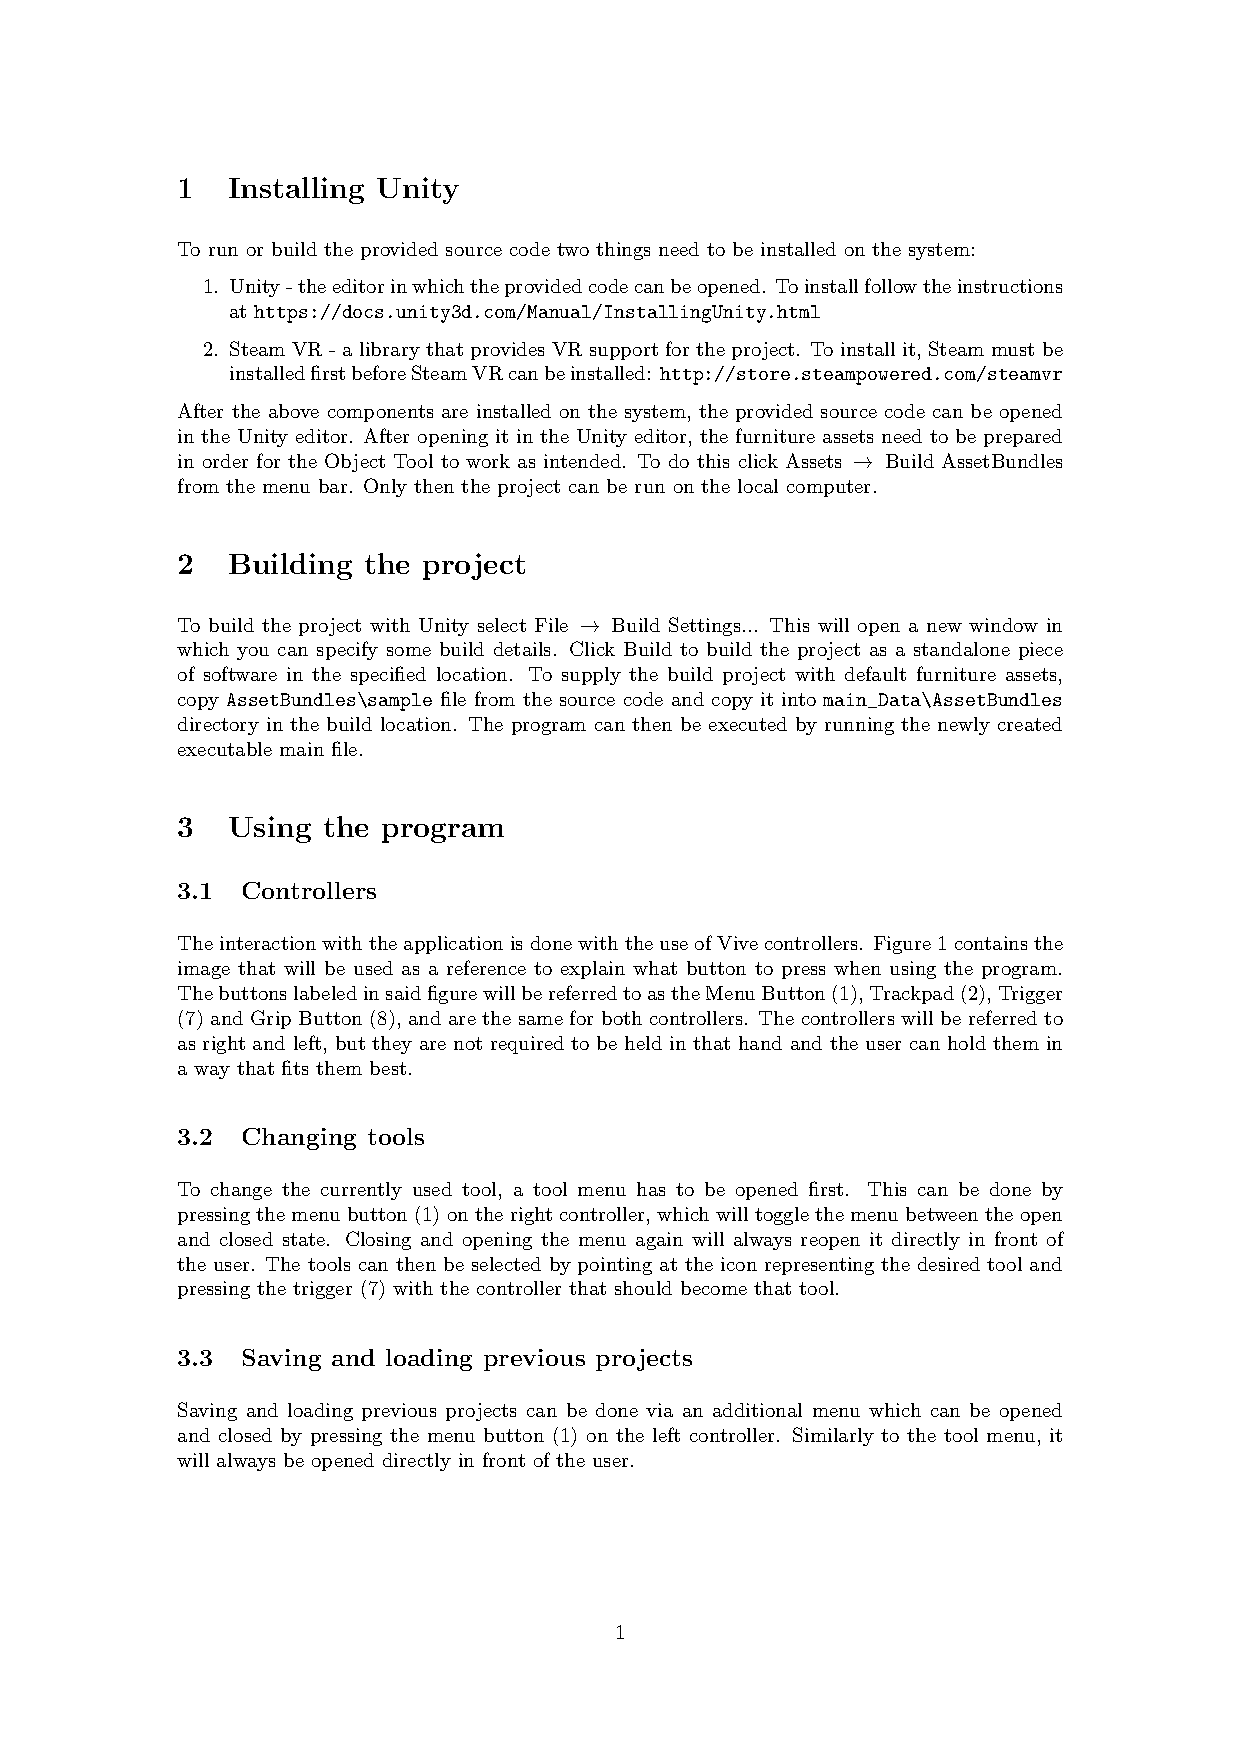
\includepdf[pages={1-3}, templatesize={16cm}{25.5cm}, frame=true]{Appendix/cs407_user_guide.pdf}

\chapter{Project Specification}
\label{app:old_spec}

The following 13 pages are the original specification submitted to the department as part of the first deliverable for the project.

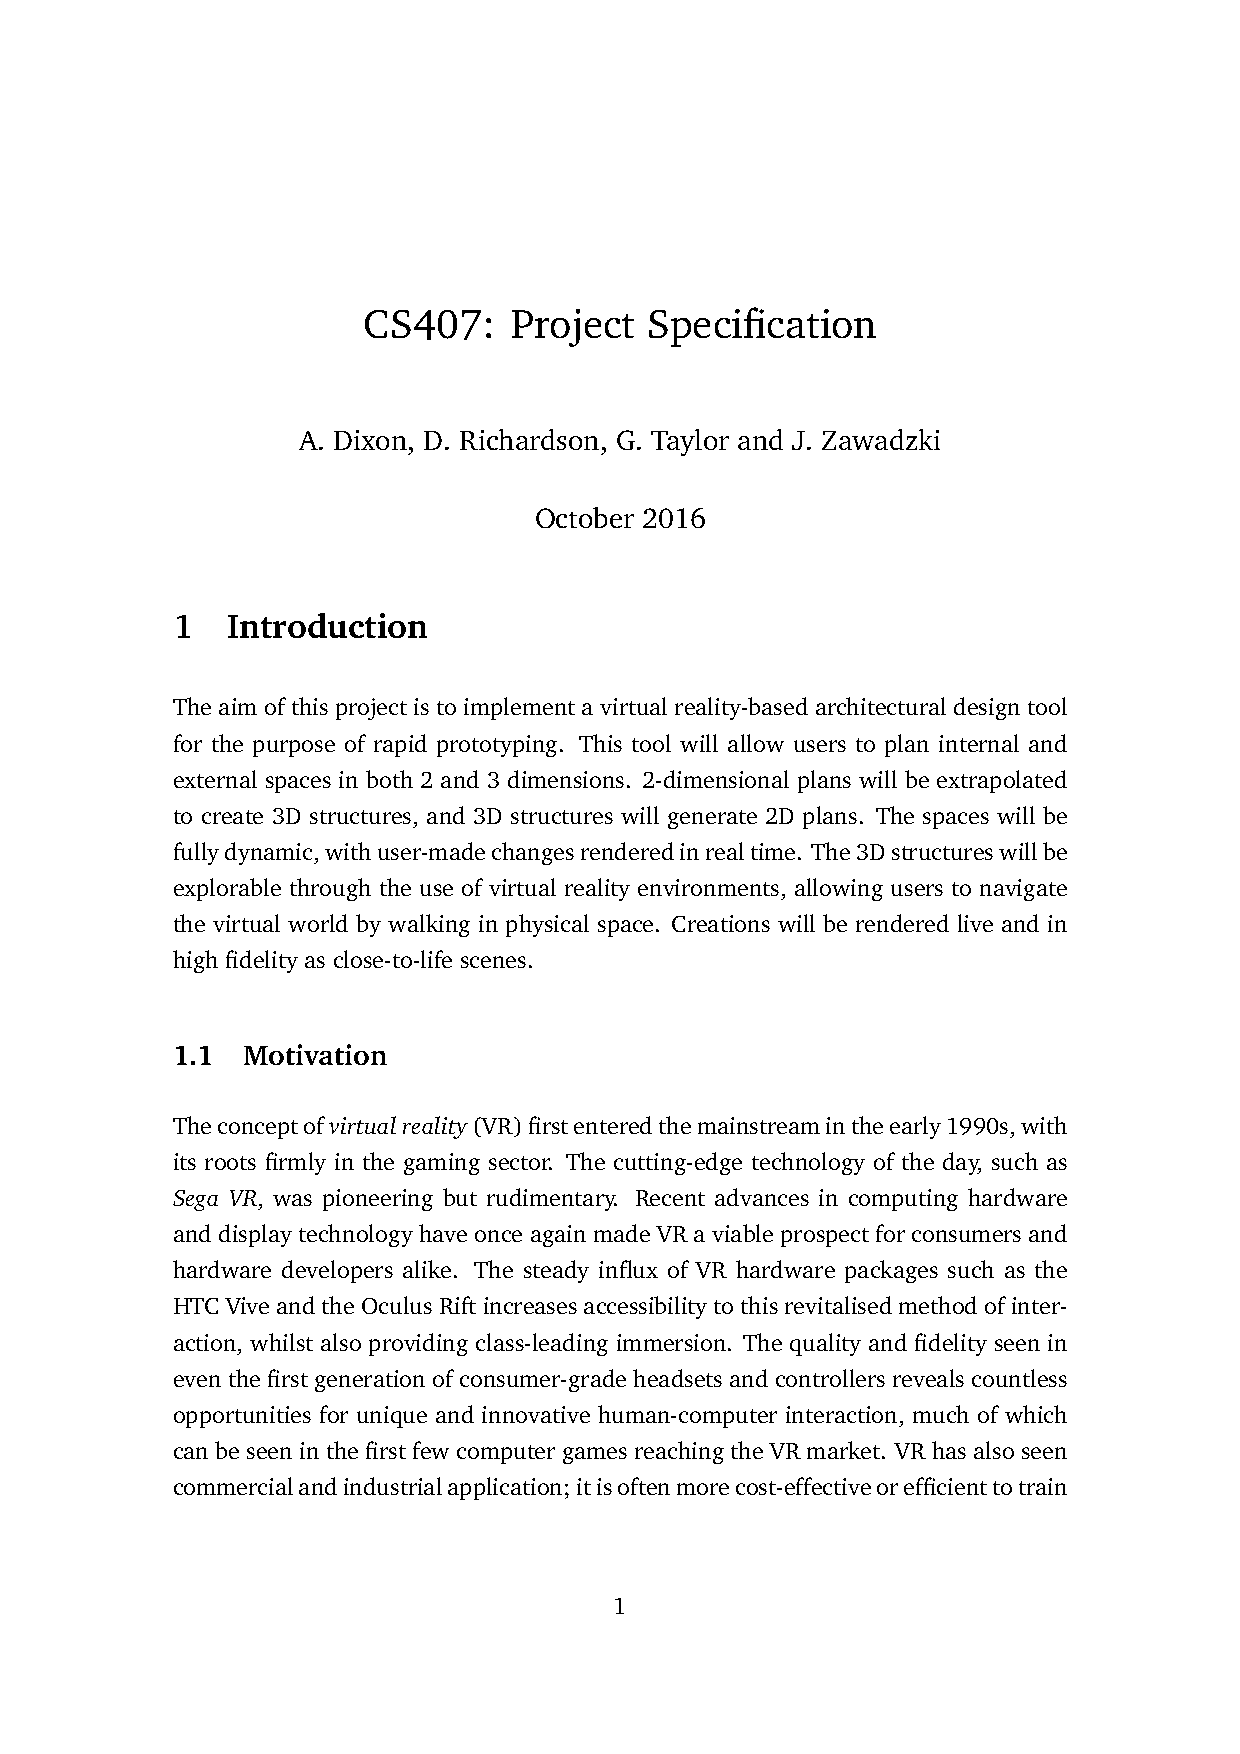
\includepdf[pages={1-13}, templatesize={16cm}{25.5cm}, frame=true]{Appendix/4th_year_spec.pdf}


\backmatter

\printbibliography
\addcontentsline{toc}{chapter}{Bibliography}

\end{document}
